\documentclass[12pt]{support/thcolognethesis} 

\usepackage{amssymb}

\title{Optimierung von Augmented Reality Anwendungen durch die Berücksichtigung von Tiefeninformationen mit Googles Project Tango}

\degree{Masterthesis}

\author{Steffen Tröster}

\college{
	Technischen Hochschule Köln\\
    Ingenieurwissenschaftliches Zentrum\\
    Fakultät für Informations-,\\
    Medien- und Elektrotechnik}

\course{Technische Informatik (Master)}

\company{inovex GmbH}  

\firstExaminer{Prof. Dr. Hubert Randerath}
\firstExaminerLocation{Technische Hochschule Köln}
\secondExaminer{Prof. Dr. Martin Eisemann}
\secondExaminerLocation{Technische Hochschule Köln}

\degreedate{Köln, im \monthyeardate\today}
	
\begin{document}

\baselineskip=18pt plus1pt

\setcounter{secnumdepth}{3}
\setcounter{tocdepth}{3}

\maketitle                 

% Die eidesstattliche Erklärung mit Unterschrift
\thispagestyle{empty}
\subsubsection*{Fakultät für Informations-, \\Medien- und Elektrotechnik}

\vspace{0.4cm}

\section*{Masterarbeit}

\vspace{0.6cm}
   
Thema: \\ 
\textbf{Optimierung von Augmented Reality Anwendungen \\
durch die Berücksichtigung von Tiefeninformationen mit \\
Googles Project Tango} \\ 

\vspace{.5cm}

\noindent Name, Vorname: Tröster, Steffen \\
Anschrift: Münchener Straße 29, 51103 Köln \\
Matrikelnummer: 11075591 \\
Studiengang: Technische Informatik (Master) \\

\noindent Erstprüfer:	Prof. Dr. Hubert Randerath \\
Zweitprüfer: Prof. Dr. Martin Eisemann \\

\noindent Anfertigungszeitraum: 10.11.2015 \\
Fertigstellung/Abgabedatum: 11.04.2016 \\



\section*{Erklärung der Urheberschaft}

Ich erkläre an Eides statt, dass ich die vorgelegte Abschlussarbeit 
selbständig und ohne fremde Hilfe verfasst, andere als die angegebenen 
Quellen und Hilfsmittel nicht benutzt und die den benutzten Quellen 
wörtlich oder inhaltlich entnommenen Stellen als solche kenntlich 
gemacht habe.


\vspace{2cm}
\hspace{2cm} Ort, Datum \hfill Unterschrift \hspace{2cm}
\begin{abstract}
\setlength{\parskip}{1em}

Project Tango ist eine neue mobile Plattform des Google Advanced Technology and Project (ATAP) Teams, die in der Lage ist, Bewegungsverfolgung, Tiefenwahrnehmung und Umgebungswiedererkennung auf Smartphones und Tablets anbieten zu können. Durch die kontinuierliche Bestimmung der relativen Geräteposition eignet sich die Plattform besonders für dreidimensionale Augmented Reality (AR) Anwendungen. Die Illusion dieser AR Anwendungen wird besonders dann gestört, wenn sich reale Objekte in einer Szene räumlich vor virtuellen Objekten befindet und diese virtuellen Objekte nicht entsprechend ausgespart werden. 

Diese Arbeit stellt daher drei Überdeckungsverfahren vor, mit denen diese Überlagerung der virtuellen Objekte mit Hilfe der Tiefenwahrnehmung von Project Tango und des Z-Buffer Algorithmus realisiert werden kann. Die Tiefeninformationen für den Z-Buffer werden hierfür zum einen direkt aus den Sensordaten und alternativ mit einer TSDF Rekonstruktion und einer selbst zusammengestellten Ebenen Rekonstruktion bestimmt. Außerdem wird auf einen zusätzlichen Ansatz eingegangen, der zur Verbesserung dieser Tiefeninformationen die Bildinformationen der Farbkamera durch den Guided Filter berücksichtigt. Diese Mechanismen werden im Laufe der Arbeit prototypisch umgesetzt und gegenübergestellt. 

\setlength{\parskip}{0em}
\end{abstract}
\selectlanguage{english}
\begin{abstract}
\setlength{\parskip}{1em}

Project Tango is a new mobile platform by Google’s Advanced Technology and Projects (ATAP) Teams, which brings Motion Tracking, Depth Perception, and Area Learning to mobile devices. With Project Tango, Google is providing a technology to tablets and smartphones for building virtual reality (VR), indoor navigation, precise measurement and augmented reality applications. The focus of this document lies mainly upon augmented reality applications. Although you can build an effective 3D AR illusion with the continuous device motion tracking, there is still a problem, that the scenes virtual object cannot be occluded by real objects when they are in foreground.

Since the Project Tango platform is offering a continues depth perception of the current viewport, this depth information can be used to solve the missing occlusion issue. This work is introducing three approaches to enable an augmented reality occlusion by real objects. Additionally an approach will be discussed to optimize the depth occlusion by taking the color information by the device’s camera into account. These methods will also get implemented with the development kit, tested, compared and evaluated concerning their applicability.

\setlength{\parskip}{0em}
\end{abstract}
\selectlanguage{ngerman}




\begin{romanpages}         
\tableofcontents            
\end{romanpages}          

% Einleitung
\chapter{Einleitung}

Project Tango ist eine neue mobile Plattform des Google Advanced Technology and Projects (ATAP) Teams, welche Bewegungsverfolgung, Tiefenwahrnehmung und Umgebungswiedererkennung auf mobilen Endgeräten realisiert.

\begin{quotation}
\enquote{Project Tango combines 3D motion tracking with depth sensing to give your mobile device the ability to know where it is and how it moves through space.}  \citep{Proje19:online}
\end{quotation}

Diese Verfügbarkeit dieser Echtzeitdaten ermöglicht viele verschiedene neue Einsatzmöglichkeiten auf mobilen Endgeräten wie Smartphones und Tablets. Typische Einsatzszenarien dieser Plattform sind die Indoor Navigation, die Vermessung der Umgebung sowie andere Anwendungen im Bereich Virtual und Augmented Reality. Der Fokus dieser Forschungsarbeit liegt hier in dem Anwendungsbereich der dreidimensionalen Augmented Reality (AR). 

Die Anwendungsgebiete für Augmented Reality (dt. Erweiterte Realität) sind sehr vielseitig und liegen in der Medizin, der Unterhaltungsindustrie, Bildung und in vielen weiteren Industriezweigen. Eine barrierefreie Navigationshilfe, Einblendungen für die persönliche Assistenz, kontextsensitive Projektionen und Computerspiele sind Beispiele für typische Anwendungen, die durch AR umgesetzt werden können. 

Für die erfolgreiche Umsetzen einer Augmented Reality Anwendung, müssen die Kameraeigenschaften, wie Brennweite, Verzerrung und die Position der Kamera zu jeder Zeit und idealerweise in Echtzeit bekannt sein. Sensoren wie Kompass, INS (Trägheits\-navigations\-system) oder GPS können zwar eine grobe Lokalisierung ohne bekannte Merkmale im Raum ermöglichen, führen aber langfristig zu Fehlern, wenn keine optischen Referenzen gegeben sind. Mit Hilfe von der Bewegungsverfolgung durch Project Tango kann diese Lokalisierung der Kamera und somit die korrekte Positionierung von virtuellen Objekten im Raum deutlich zuverlässiger, in Echtzeit und ohne vordefinierte Merkmale im Raum realisiert werden. Project Tango eignet sich daher sehr gut für die Umsetzung und den Einsatz von AR Anwendungen.

\section{Augmented Reality Optimierung}

Um eine für den Betrachter effektive und optimierte Augmented Reality Anwendung umsetzen zu können, benötigt man laut \citet{azuma2001recent} die Möglichkeit mehr Informationen über relevante Objekte im realen Raum ermitteln zu können. Durch diese Informationen könnte dem Nutzer zum Beispiel eine Interaktion mit realen Objekten ermöglicht werden oder anhand optischer und semantischer Einordnung der Umgebung passende Funktionen angeboten werden. 

Hinsichtlich der zuletzt erwähnten Kontextsensitivität existieren viele Ansätze, basierend auf optischen Merkmalen der Umgebung. So kann zum Beispiel ein optisches Tracking von realen Objekten, wie von \citet{lee2008hybrid} beschrieben, umgesetzt werden. Project Tango nutzt bereits optische Merkmale, um eine Positionsverfolgung oder das Lernen der Umgebung umzusetzen. Wären diese Merkmale für den Entwickler als Schnittstelle verfügbar, könnte man mit diesen Informationen solche kontextsensitiven Anwendungen umsetzen. Der Fokus soll in dieser Arbeit jedoch nicht auf den optischen Merkmalen sondern auf den Tiefeninformationen, die Project Tango durch den eingebauten Tiefensensor in Form einer Pointcloud liefern kann, liegen.

Ein sinnvoller Einsatz von Augmented Reality Anwendungen besteht darin, virtuelle Objekte in eine echte Szene zu projizieren. Dabei überlagert die Projektion des virtuellen Objekts das aktuelle Kamerabild oder den aktuellen Sichtbereich und erwirkt dadurch den Anschein, als ob sich das virtuelle Objekt wirklich in der Szene befindet. Dieser Effekt funktioniert solange erfolgreich, bis ein reales Objekt sich räumlich vor das virtuelle Objekt bewegt und die zu erwartende Überlagerung des virtuellen Objekts nicht erfolgt. Diese fehlerhafte Darstellung durch eine fehlende Überdeckung ist in Abbildung \ref{fig:occlusion-problem} zu erkennen. 

\begin{figure}[h]
  \centering
	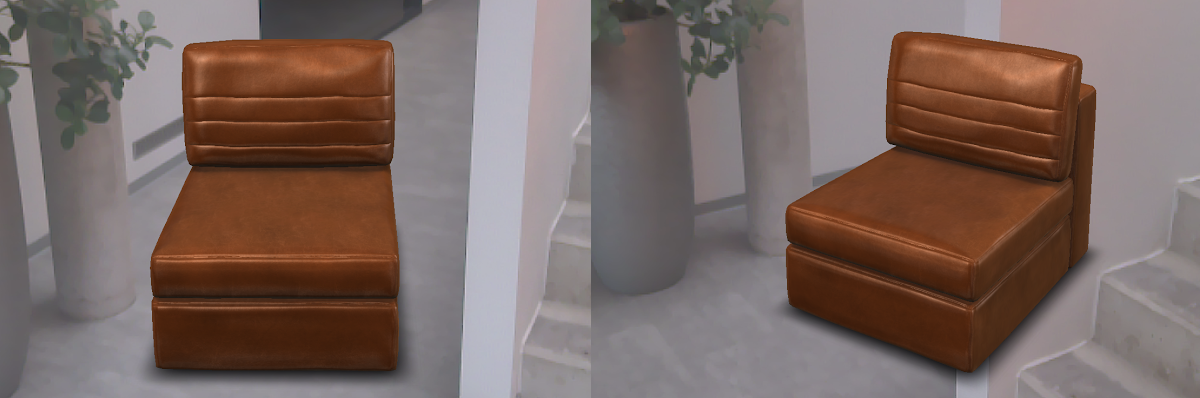
\includegraphics[width=1.0\textwidth]{content/images/occlusion-problem.png} 

  \caption{AR Projektion mit Project Tango - Links: Erfolgreiche Projektion. Rechts: Fehlerhafte Darstellung ohne Überdeckung.}
  \label{fig:occlusion-problem}
\end{figure}

Die Verfügbarkeit der Tiefeninformationen bei Project Tango könnte die Interaktionen oder Darstellungen in einer Augmented Reality Anwendung präziser an die echten räumlichen Gegebenheiten anpassen. Es existieren zum Beispiel prototypische Anwendungen, in denen virtuelle Markierungen passend an echten Objekten im virtuellen Raum positioniert werden können, indem sie auf die aktuellen Tiefeninformation des Sichtbereichs zurückgreifen. Eine weitere Idee ist es, Überlagerungen virtueller Objekte ermitteln zu können, an denen sich reale Objekte im Vordergrund befinden.

\section{Zielsetzung und Vorgehen}

Diese Arbeit will die Fragestellung beantworten, durch welche Verfahren mithilfe der Tiefeninformationen von Project Tango, automatisch und in Echtzeit die Überdeckung virtueller Objekte mit realen Objekten in einer Augmented Reality Szene realisiert werden kann. Dabei soll Project Tango als autonomes System betrachtet werden, welches diese Problemstellung selbstständig und mit den eingeschränkten Ressourcen dieser mobilen Plattform lösen soll.

Hierzu sollen zunächst bestehende Verfahren zur Bestimmung einer Augmented Reality Überdeckung durch eine Literaturrecherche gefunden werden. Diese Verfahren sollen dabei auf Ihre Anwendbarkeit mit der Project Tango Hardware überprüft werden. Sollten sich aus der Recherche weitere Ideen ergeben, wie speziell auf der Project Tango Hardware eine Überdeckung umgesetzt oder verbessert werden kann, sollen diese mit in die Arbeit eingebunden werden. Eine Idee könnte zum Beispiel sein, auch das Farbbild der normalen Kamera von Project Tango in die Optimierung der virtuellen Überlagerung einfließen zu lassen. Die identifizierten Verfahren sollen hiernach entsprechend implementiert werden, um sie darauf folgend in einer Testumgebung gegenüber zu stellen.

Strukturell wird in dieser Arbeit in Kapitel \ref{sec:thema} erst einmal auf die thematischen Grundlagen zu Augmented Reality und Project Tango eingegangen. Hier werden auch die existierenden Verfahren zur AR Überdeckung angesprochen. Unter Kapitel \ref{sec:algorithms} sind theoretische Grundlagen zu finden, die bei der späteren Umsetzung verschiedener Verfahren angewendet werden. Kapitel \ref{sec:optimization} beinhaltet die Argumentation und Beschreibung der gewählten Verfahren, welche unter Kapitel \ref{sec:implementation} auf der Project Tango Hardware umgesetzt werden. In Kapitel \ref{sec:evaluation} werden die vorliegenden Umsetzung in einem Testszenario gegenübergestellt, um eine Aussage treffen zu können, welcher Ansatz auf der Hardware oder für einen bestimmten Einsatz gut funktionieren könnte.




% Thematische Vorbemerkung
\chapter{Thematische Vorbemerkung} \label{sec:thema}

Im ersten Teil dieses Kapitels werden zunächst einmal die Grundlagen zu Augmented Reality beschrieben, wie diese Technologie einzuordnen ist, welche technischen Anforderungen ein Augmented Reality System hat und wo typische Einsatzszenarien liegen. Außerdem wird hier auf den aktuellen Stand der Forschung bezüglich der Bestimmung von Überdeckungen in einem Augmented Reality System eingegangen. Hiernach wird näher auf Googles Project Tango eingegangen, welche Konzepte angewendet werden und wie diese Technologie im Bereich Augmented Reality einzuordnen ist. \\


\section{Augmented Reality}

Augmented Reality (AR) ist eine Klasse aus dem Realitäts-Virtualitäts-Kontinuum von \cite{milgram1995augmented}, welches in Abbildung \ref{fig:virtual-continuum} abgebildet ist. Diese Klasse beschreibt die Darstellungen von realen und virtuellen Informationen in einer Repräsentationsform, wobei hier reale und virtuelle Objekte in einer realen Umgebung kombiniert dargestellt werden können. Diese virtuellen Objekte sind in der realen Umgebung idealerweise fest lokalisiert und fügen sich somit in das reale Erscheinungsbild ein. Typischerweise sind AR Anwendungen interaktiv, und stellen die virtuellen Objekte in Echtzeit und dreidimensional in der realen Welt dar. Für die Definition von AR Anwendungen gibt es zudem keine Limitierung für die Darstellungstechnologie, wie zum Beispiel das Project Tango Tablett oder einem Head-Mounted-Display. AR beschränkt sich zudem nicht auf den angesprochenen Sinn - so sind zum Beispiel AR Anwendungen mit visueller, taktiler oder sogar olfaktorischer Umsetzung möglich.

\begin{figure}
  \centering
	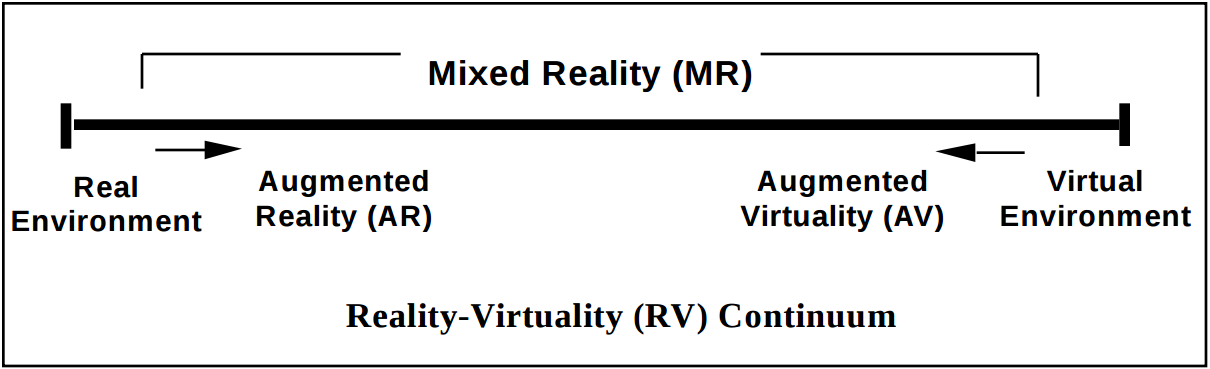
\includegraphics[width=0.85\textwidth]{content/images/theory/virtual-continuum.png} 
  \caption{Vereinfachte Darstellung des Realitäts-Virtualitäts-Kontinuum von \citet*{milgram1995augmented}}
  \label{fig:virtual-continuum}
\end{figure}


Virtuel Reality (VR) oder auch Virtual Environment hingegen kapselt sich von der realen Umgebung ab und bietet Interaktionen in reinen virtuellen Umgebungen. Diese rein virtuelle Darstellung konnte sich im Gegensatz zu Augmented Reality deutlich schneller Entwickeln, da die technologischen Anforderungen an AR deutlich höher sind. \citep{van2010survey}

\subsection{Technische Anforderungen}

Dieser Abschnitt widmet sich den technischen Anforderungen an Augmented Reality, indem die potentiellen Display Technologien beschrieben werden, mögliche Trackingverfahren zur Ermittlung der Betrachtungsposition erläutern werden und auch die Systeme behandelt werden, mit denen ein Nutzer mit den virtuellen Darstellungen interagieren kann.

\subsubsection{Display Technologie}

Der erste wichtige Teil der technologischen Anforderungen an AR sind visuelle Anzeigen (visual displays), die neben der Möglichkeit eines dreidimensionalen Renderings, welches hier aus der Virtual Reality vorausgesetzt werden soll, weitere Charakteristika mit sich bringen. Nach \citet{van2010survey} lassen sich diese Technologien zunächst in je drei Arten der Darstellung und Positionierung unterteilen.

Die einfachste und günstigste Art der visuellen Darstellung in AR ist \enquote{video see-through}, wodurch die reale Umgebung durch eine Video Aufnahme ersetzt wird und die virtuellen Objekte digital in die Video Aufnahme gerendert werden. Das bietet die Möglichkeit Objekte aus der realen Umgebung zu entfernen oder zu ändern oder, anhand der Luminanz Information vom Video, das Rendering der virtuellen Objekte entsprechend an die Realität anzupassen. Anwendung findet diese Technologie typischerweise in Tablets, Smartphones oder Head-Mounted-Displays.

Die nächste Möglichkeit zur Darstellung ist \enquote{optical see-through}. Hier werden die virtuellen Objekte durch transparente Spiegel in das Sichtfeld des Betrachters gebracht. Anders als bei \enquote{video see-throught} bleibt die reale Auflösung für die visuelle Aufnahme des Betrachtes gleich und es können zudem nur Latenzprobleme bei dem Rendering der virtuellen Objekte und nicht bei der Darstellung der realen Umgebung auftreten. Auf der anderen Seite besteht bei dieser Technologie das Problem, dass die Darstellung von virtuellen Objekten nicht kräftig genug ist, um die reale Umgebung auf Grund von der transparenten Darstellungsoberfläche komplett auszublenden. Typische Geräte dieser Technologie sind Headmounted Displays wie Google Glass\footnote{\url{https://developers.google.com/glass/} (23.02.2016)} oder stationäre Geräte wie der HoloDesk\footnote{\url{http://research.microsoft.com/en-us/projects/holodesk/} (23.02.2016)}.

Die dritte Möglichkeit ist die projizierte Darstellung, in der die Augmented Reality Überlagerung auf die realen Objekte projiziert werden. Diese Darstellung ermöglicht die Abdeckung vom gesamten Sichtfeld des Betrachters, benötigt aber eine entsprechende Kalibrierung oder eine Strukturwahrnehmung bei Umgebungsänderungen.

Neben der Art der Darstellung können die Display Technologien laut \citet{azuma2001recent} anhand Ihrer Positionierung klassifiziert werden. Man unterscheidet zwischen am Kopf befestigten Displays (head-mounted), tragbaren Displays (hand-held) und räumlich positionierten Displays. Zu jeder dieser Displayarten gibt es wiederum unterschiedliche technische Umsetzungen mit ihren spezifischen Vor- und Nachteilen bezüglich ihrer Anwendungsszenarien.

\subsubsection{Tracking Technologien}

Um eine virtuelle Projektion im realen Raum auf nicht stationären Displaytechnologien zu realisieren muss die Position und gegebenenfalls relative Positionsänderung des Displays bestimmt werden, auch \enquote{augmented reality registration} genannt. Man spricht dabei üblichweise von den \enquote{six degrees of freedom (6DOF)}, der Position im Raum (x, y, z) und der Orientierung (yaw, pitch, roll). 

Frühe Techniken für die Registrierung benötigten üblicher Weise eine speziell vorbereitete Räumlichkeit, denn sie basierten auf mechanischen, magnetischen oder Ultraschall Sensoren um die Position zu bestimmen. Diese Sensoren sind zwar immer noch im Einsatz und bilden auch den Grundstein für die AR und VR Forschung, sind aber praktisch gesehen zu komplex und aufwändig für die meisten Anwendungsfälle. \citep{van2010survey} 

Für ein grobes Positions-Tracking, vor allem auch außerhalb von Gebäuden wird GPS genutzt. Für großräumige Anwendung ist GPS, mit einer Varianz von 10-15 Metern und in Kombination mit einem Kompass, durchaus praktikabel. Als Beispiel reicht diese Genauigkeit aus, um sichtbare Flugzeuge oder Sterne visuell aufzubereiten. Innerhalb von Gebäuden basiert die grobe Positionierung laut \citet{van2010survey} oft auf verfügbaren Wifi Access Points oder RFID Markern. \citet{lamarca2005place} demonstrieren hierzu auch die Möglichkeit diese Idee für grobe Lokalisation außerhalb von Gebäuden einzusetzen.

Optische Tracking Verfahren, basierend auf Bildverarbeitung, bieten laut \citet{van2010survey} deutlich genauere Resultate als die zuvor beschriebenen Verfahren. Es gibt hier viele verschiedene sensorische Ansätze ein optisches Tracking zu realisieren. Frühe verfahren, wie die von \citet{dunston2008identification} oder \citet{narzt2006augmented}, nutzten Passmarker (fiducial marker) oder Licht emittierende LEDs in einem vordefinierten Modell, um zwischen aufgenommenen Bildern die Marker oder LEDs zu detektieren und zusammengehörige zwischen den Bildern zu finden, um daraus eine Kameratransformation zu berechnen. Neue Verfahren ohne Marker, wie das sogenannte \enquote{visual odometry} von \citet{nister2004visual}, nutzen Techniken zur Feature Detection und Matching um Referenzen und Bewegungen zwischen aufgenommenen Bildern zu bestimmen.

Viele kommerzielle und erfolgreiche Tracking Verfahren beruhen jedoch auf hybride Ansätze, in denen die Informationen mehrerer Sensoren kombiniert werden, um potentielle Messfehler eines Sensors oder einer Methodik auszuschließen. So werden zum Beispiel Neigungssensor, Kompass und Gyroskop mit einem optischen Verfahren kombiniert, um ein Tracking der sechs Freiheitsgrade zu optimieren. Diese Erweiterung des optischen Verfahrens wird auch \enquote{visual-inertial odometry} genannt. \citep{van2010survey}

\citet{azuma2001recent} erwähnt an dieser Stelle auch die Kalibrierung der Sensoren, die für ein präzises Registrieren nötig ist. So müssen zum Beispiel die Linseneigenschaften der Kamera für optisches Tracking bekannt sein, damit die Verfahren mit Krümmungen, Verzerrungen und den perspektivischen Eigenschaften der Kamera umgehen können. Diese Informationen sind auch bei video see-through Displays für ein korrektes Projizieren der 3D Objekte wichtig. Zudem wird erwähnt, dass man Messfehlern oder Drifts der Position zum Beispiel mit der Zunahme von Gyroscop Informationen entgegenwirken kann, indem man Ereignisse wie einen Schritt des Nutzers einfließen lässt. \citep{azuma2001recent} 

\subsubsection{Interaktions Technologien} \label{sec:ar-interaction}

Neben den Display und Tracking Technologien ist es notwendig dem Nutzer andere Interaktionsmöglichkeiten anzubieten, da in der Regel das klassische zweidimensionale WIMP Paradigma (Windows, Icons, Menus and Pointer) im dreidimensionalen Kontext von AR keine ausreichende Gebrauchstauglichkeit bietet. Dennoch müssen die Interaktionstechnologien in Augmented Reality die üblichen Interaktionen wie aus WIMP unterstützen. Dazu gehören zum Beispiel das Auswählen, Positionieren und Drehen von virtuellen Objekten, das Zeichnen von Pfaden oder Flugbahnen, sowie die Eingabe von Quantitativen Werten oder Texten. \citep{van2010survey} 

Frühe Augmented Realilty Systeme nutzen einfache Trackballs, Trackpads, Touchscreens oder Gyroscopmäuse für eine zweidimensionale Interaktion mit dem System. Später wurden dreidimensionale Equivalente eingeführt, wie 3D Mäuse oder Stifte, die eine dreidimensionale Interaktion ermöglichen. Diese Greifbaren Schnittstellen werden auch TUIs genannt (Tangible User Interface) und ermöglichen eine unidirektionale Interaktion mit dem System. Zudem wurden auch TUIs mit haptischen Feedback eingeführt, wie zum Beispiel die 3D Maus PHANTOM. \citep{van2010survey} 

Eine weitere Art der TUIs sind laut \citet{azuma2001recent} Gegenstände, mit denen der Nutzer natürlich interagieren kann und die vom System optisch erfasst werden, um die Positionsänderung der Objekte anhand von Markern oder anderen optischen Merkmalen zu bestimmen. Somit kann ein Nutzer, zum Beispiel, für die virtuelle Einrichtung eines Raums, die Möbel mit Hilfe eines echten Gegenstands im Raum verschieben. 

Nicht taktile Systeme verwenden meist optische Aufnahmen, um Gesten der Hände, des gesamten Körpers oder die Blickrichtung des Nutzers erkennen zu können. Für die Realisierung werden dazu Kameras am Körper oder im Raum verwendet. Außerdem ist es möglich Spracherkennung in die Interaktion mit einfließen zu lassen, um eine möglichst authentische Interaktion zu bieten. Wie auch bei den Tracking Technologien existieren hierbei Hybride Systeme, die verschiedene Interaktions Technologien kombinieren. \citep{van2010survey} 

\subsection{Anwendungsbereiche}

Über die Jahre habe Wissenschaftler immer mehr Bereiche identifiziert, die von der Anwendung von Augmented Reality profitieren können. \citet{van2010survey} nennt dazu als Erstes Einsatzgebiet die persönliche Assistenz, in der AR Systeme eingesetzt werden können, um zum Beispiel mit Hilfe von Brillen (zum Beispiel der Google Glass) Namen der sichtbaren Personen anzuzeigen, die Navigation in unbekannten Regionen einzublenden oder beim Sightseeing Kontext relevante Informationen im Sichtfeld anzuzeigen. 

Neben der persönlichen Assistenz können auch Anwendungen in der Industrie laut \citet{van2010survey} von AR profitieren. Es lassen sich zum Beispiel virtuelle Designumgebungen umsetzten, die es ermöglichen ein Auto in Lebensgröße zu Gestalten. Auch bei der Fertigung und Konstruktion können den Arbeitern unterstützende Informationen angezeigt werden. So werden zum Beispiel zu erledigende Schweißstellen hervorgehoben oder der Plan zur Konstruktion entsprechend eingeblendet. Oder für die Instandhaltung komplexer Maschinen kann ein AR System dem Nutzer eine Art Röntgenblick Hinweise auf potentielle Schwachstellen liefern. Auch in der Rüstungsindustrie existieren Anwendungsgebiete für Augmented Reality Systeme. So können zum Beispiel Gefechte für eine Kampfausbildung besser simuliert werden. \citep{azuma2001recent} 

Für Anwendungsbereiche in der Medizin ist ein sehr genaues Tracking der Freiheitsgrade erforderlich, da AR in der Chirurgie und Behandlung von Patienten Anwendung findet. Erstellte Röntgenbilder oder Ultraschallbilder können hierdurch, anstatt auf einem separaten Monitor, direkt auf die entsprechende Körperstelle projiziert werden, wodurch gegebenenfalls eine genauere Untersuchung oder Behandlung möglich ist. \citep{van2010survey} 

Augmented Reality wird auch im Entertainment Sektor eingesetzt. Videoübertragungen von Sportereignissen werden heutzutage oft durch zusätzliche Informationen angereichert. So erhalten zum Beispiel American Football Spiele dynamische Spielfeld Begrenzungen. Auch die Werbeeinblendungen am Rand des Spielfelds können entsprechend dem Gebiet der Ausstrahlung ausgetauscht werden. \citep{azuma2001recent} 

Ein weiteres großes Anwendungsgebiet für Augmented Reality sind laut \citet{azuma2001recent} Computerspiele, in denen es möglich ist, in einer beliebigen Umgebung Objekte eines Spiels im Raum zu platzieren und mit Ihnen entsprechend zu interagieren. Die natürlichere Interaktion, gegenüber herkömmlichen Spielplattformen, und die Nutzung in einer persönlichen Spielumgebung führt zu einem intensiveren Spielerlebnis. 

In der Bildung für Schulen oder Museen ist es auch mögliche AR Systeme einzusetzen. Zur Vermittlung von geometrischen oder mathematischen Grundlagen gibt es die Möglichkeit der kollaborativen und interaktiven Visualisierung von Körpern, an denen etwa Parameter manipuliert werden, um danach Ihre Eigenschaften besser beobachten und nachvollziehen zu können. \citep{van2010survey} 

\subsection{Einschränkungen und Probleme}

Die frühen Augmented Reality Systeme sind auf Grund ihrer Größe sehr unhandlich und mobil daher nur mit großem Aufwand anwendbar. Durch die Verfügbarkeit mobiler und performanter Endgeräte ist ein mobiler Einsatz wiederum ermöglicht worden. Jedoch besitzen die aktuellen Geräte wie Smartphones oder Tabletts nicht die entsprechende Sensorik für ein präzises Tracking der sechs Freiheitsgrade. \citet{van2010survey} weisen zudem darauf hin, dass die Registrierung der Tiefe für die Anwendung von Überdeckungen oder korrekter Positionierung bei einer Interaktion ein komplexes Problem sei. Wie in Kapitel \ref{sec:theory_project_tango} zu finden geht Project Tango dieses Problem der Sensorik entsprechend an und versucht Schnittstellen zu bieten, um sowohl das Tracking zu ermöglichen und Tiefeninformationen über die aktuelle Szene zu liefern. 

Eine weitere erwähnenswerte Problematik ist neben der sensorischen Themen von Augmented Reality die Herangehensweise zur Gestaltung der Nutzeroberflächen für AR. Denn die UI Konzeption gestaltet sich, laut \citet{azuma2001recent}, als schwierig. Die Anreicherungen durch Augmented Reality führt schnell dazu, dass das Sichtfeld überladen wirkt. Jedoch soll dem Nutzer immer die Informationen zur Verfügung gestellt werden, die gegebenenfalls kontextsensitiv und relevant sind. Diese Angesprochenen Faktoren führen aktuell bei Augmented Reality Anwendungsgebieten noch zu einer geringen Akzeptanz der Endverbraucher.

\subsection{Realisierung von Augmented Reality Über\-deckungen} \label{sec:ar-occlusion}

Es gibt einige Verfahren und Ansätze, um eine Überlagerung in Augmented Reality Szene zu realisieren. \citet{wloka1995resolving} bilden hierfur den Grundstein für die verschiedenen existierenden Methoden. Sie stellen in Ihrer Arbeit ein Verfahren vor, welches mit Bildern aus einer Stereo Kamera ein Stereomatching durchführt und dadurch ein Tiefenbild generiert. Dieses Tiefenbild führt in dem Renderingprozess mit Hilfe des Z-Buffer Algorithmus (beschrieben in Kapitel \ref{sec:z-buffer}) zum Ausschluss von Teilen der virtuellen Objekte, die von realen Objekten überlagert werden. Das Ergebnis des Stereomatchings ist in ihrer Arbeit mit gewissen Ungenauigkeiten behaftet und generiert unerwünschte Lücken in der Projektion des virtuellen Objekts. Arbeiten wie von \citet{seo2013direct}, mit neuen Tiefensensoren wie der Microsoft Kinect\footnote{Microsoft Kinect - https://dev.windows.com/en-us/kinect (04.03.16)}, erhalten durch den selben Mechanismus deutlich bessere Ergebnisse. 

Die Arbeit von \citet{breen1996interactive} nahmen diesen Ansatz von \citet{wloka1995resolving} auf und stellten die Idee vor, neben einer deutlich genaueren Überdeckung auch eine Interaktion mit realen Objekten zu realisieren. Hierfür werden virtuelle Modelle der realen Objekte in der Szene passend an der echten Umgebung und der Position der realen Objekte ausgerichtet. Dieses Vorgehen setzt jedoch voraus, dass die entsprechenden virtuellen Modelle für die realen Objekte bereits vorliegen. Nach dieser Ausrichtung wird die Tiefe der virtuellen Objekte gewonnen, um daraus, mit dem Verfahren von \citet{wloka1995resolving}, eine Überlagerung durch den Ausschluss der weiteren virtuellen Objekten der Szene zu bewirken. 

Neben den Modell basierten Verfahren existieren auch Kanten basierte Verfahren, wie das von \citet{berger1997resolving}, in dem Objektkanten auf optischer Basis mit Filtern ermittelt werden. Diese Kanten werden über mehrere Bilder verfolgt, um die Tiefeninformation der Kanten durch Epipolargeometrie und Heuristiken zu bestimmen. \citet{berger1997resolving} gewinnt darauf folgend  eine Tiefenmaske, indem er annimmt, dass Konturen, die unter einer gewissen Distanz von einander entfernt sind, zu einem Objekt gehören. \citet{klein2004sensor} erreichen mit einer, auf mobiler Hardware umgesetzten Umgebung, mit diesem Verfahren, sehr überzeugende Ergebnisse in einer vordefinierten Umgebung. Zwar verspricht dieses Vorgehen eine Kanten genaue Überdeckung virtueller Objekte, führt aber bei komplexeren Szenen, in denen die Kanten nicht mehr erfolgreich verfolgt werden oder nicht zu einem Objekt zugeordnet werden können, zu Fehldarstellungen. Außerdem werden Ausbreitungen innerhalb des Objekts, welche nicht als Kante erkannt werden können, nicht berücksichtigt.

Die letzte Variante wurde von \citet{breen1996interactive} bereits erwähnt, ist die Ermittlung der Überdeckung durch eine Rekonstruktion der Szene. Dieser Ansatz verschiebt durch das Verfahren von \citet{wloka1995resolving} die Problemstellung der AR Überdeckung in den Bereich der Echtzeit Rekonstruktionsproblematik. Bekannte Verfahren hierfür sind zum Beispiel KiniectFusion von \citet{newcombe2011kinectfusion} oder die Echtzeit Rekonstruktion von \citep{niessner2013real}. Diese sehr komplexen Verfahren sind meist auf der Grafikhardware von Desktopsystemen umgesetzt und generieren eine detaillierte Rekonstruktionen aus den Tiefeninformationen in Echtzeit. Diese Rekonstruktionen können laut \citet{newcombe2011kinectfusion} für eine Echtzeit Überdeckung in Augmented Reality Systemen dienen. Vorteilhaft bei einer Rekonstuktions basierter Überdeckung ist zudem, dass auch Interaktionen mit echten Objekten, wie bei \citet{breen1996interactive}, erfolgreich umgesetzt werden können.





\section{Project Tango} \label{sec:theory_project_tango}

Project Tango ist eine Technologie Plattform für Android Tablets und Smartphones von Google’s Advanced Technology and Projects Group (ATAP). Das Ziel dieser Plattform ist es, Motion Tracking (Positionierung), Depth Perception (Tiefeninformation/Pointcloud) und Area Learning (Lokalisierung) auf mobile Endgeräte zu bringen, um verschiedenste Anwendungs-Szenarien abzudecken. Typische Szenarien sind Indoor Navigation, Virtual Reality Anwendungen, Vermessungs- und Rekonstruktions\-software und Augmented Reality Anwendungen.

Das System ermöglicht in erster Linie ein Tracking von Positionsänderungen des Geräts im Raum und bietet somit eine genaue relative Lokalisierung. Mit Hilfe dieser Lokalisierung und der Hinzunahme von visuellen Merkmalen im Raum ist das Gerät in der Lage, seine Umgebung kennenzulernen und gegebenenfalls die Lokalisierung zu korrigieren oder aber diese in einer bereits erlernten Umgebung zu bestimmen. Zusätzlich bietet Project Tango die Möglichkeit, mit Hilfe eines Tiefensensors, eine Pointcloud der Tiefeninformation pro Bildausschnitt zu ermitteln, um Anwendungen auch räumliche Informationen bereitzustellen.  \citep{Proje19:online} 

\subsection{Geräte und Hardware}

Da das Project Tango zum Zeitpunkt der Verfassung dieser Thesis noch unter Entwicklung steht, gibt es von Google nur erste Entwickler Prototypen. Das erste Gerät \enquote{Peanut Phone} im Smartphone Format, welches in Abbildung \ref{fig:tango-device} rechts unten zu erkennen ist, wurde Anfang 2014 veröffentlicht und ein halbes Jahr später bereits durch eine neue Generation, dem \enquote{Yellowstone Tablet} ersetzt. Dieses 7\dq Tablet, zu sehen rechts oben im Bild \ref{fig:tango-device}, verfügt, wie in der Abbildung links zu erkennen, über einen Infrarot Laser Projektor, eine Fisheye Kamera und eine normale 4 Megapixel Kamera auf der Rückseite. Zudem sind, wie in aktuellen Smartphones und Tablets üblich, ein Beschleunigungssensor, Umgebungslichtsensor, Barometer, Kompass, GPS und ein Gyroskop verbaut. Das Gerät wird von einem NVIDIA Tegra K1 Prozessor betrieben und verfügt über 4GB Arbeitsspeicher. \citep{Proje19:online} Mit diesem Gerät wurden die später beschriebenen Techniken umgesetzt und evaluiert. 

\begin{figure}[h]
  \centering
	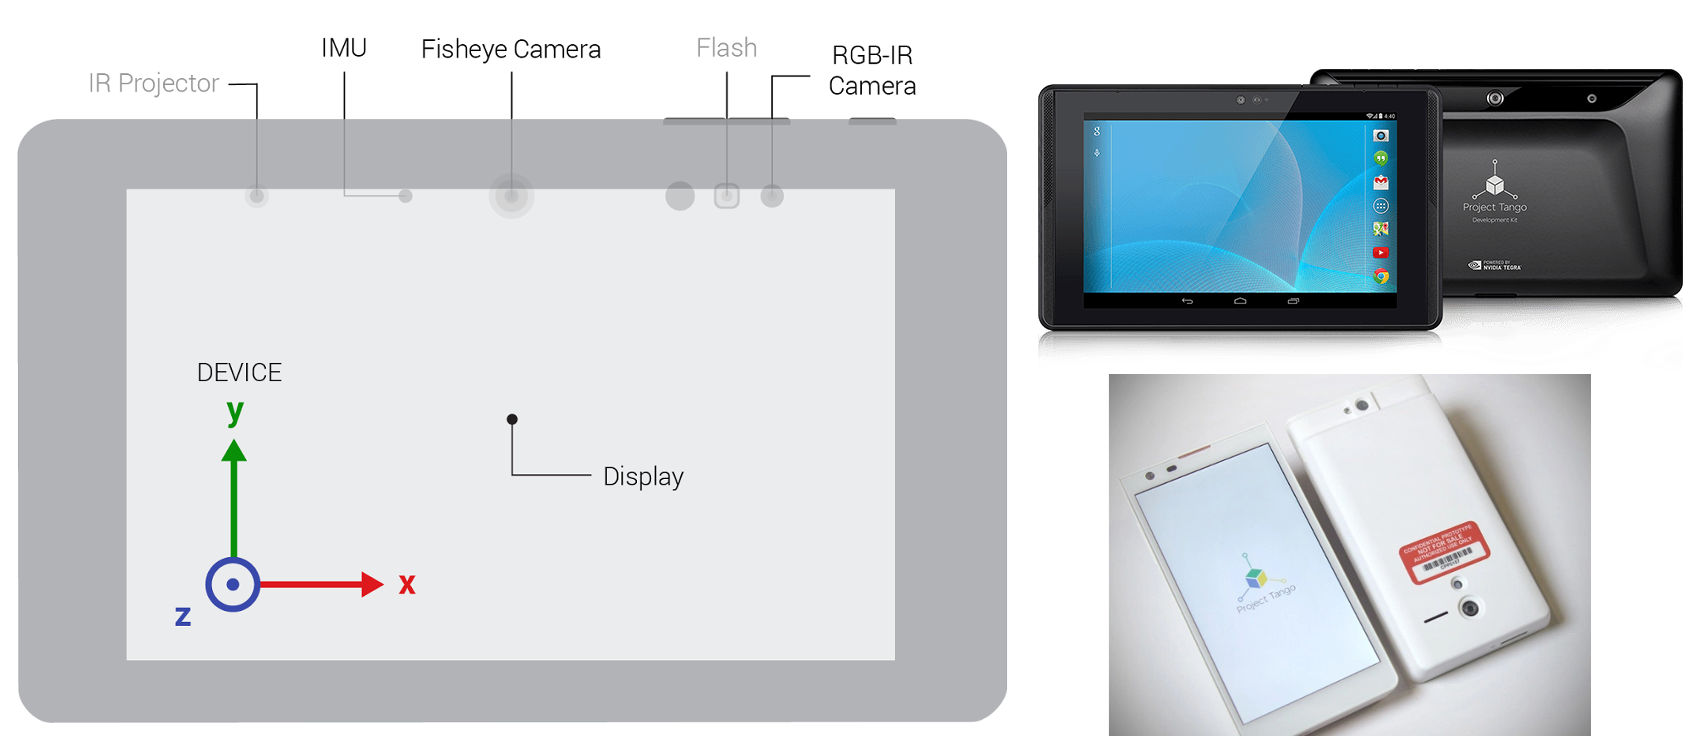
\includegraphics[width=1.0\textwidth]{content/images/theory/tango-device.png} 
  \caption{Links: schematischer Aufbau der Google Project Tango Hardware. Rechts: Das aktuelle Entwickler Gerät im Tablet Format (oben) und das alte Entwickler Gerät im Smartphone Format (unten). Übernommen von \citet{GoogleDevelopers:online}}
  \label{fig:tango-device}
\end{figure}

\subsection{Konzepte und Schnittstellen}

Generell betrachtet ist das Project Tango eine Plattform, die Computer Vision nutzt, um dem Gerät die Möglichkeit zu bieten seine relative Positionierung in der umgebenden Szene in Echtzeit zu bestimmen. Auf den Geräten kommt Googles Android Betriebsystem zum Einsatz, weshalb zu beachten ist, dass es sich bei der Plattform nur bedingt um eine Echtzeitumgebung handelt. Das liegt daran, dass der Linux Kernel keine Garantien für die zeitlich präzise Ausführung von Instruktionen auf Grund von Scheduling geben kann. Google weist daher darauf hin, dass das System als \enquote{soft-realtime} betrachtet werden sollte. Daher sollten Messergebnisse verschiedener Sensoren unter Berücksichtigung ihrer Aufnahmezeitpunkte verwendet werden. \citep{GoogleDevelopersConcepts:online} 

\subsubsection{Motion Tracking}

Um die relative Bewegung vom Start des Project Tango Systems bestimmen zu können, nutzt es \enquote{visual-inertial odometry}. \citep{GoogleDevelopersConcepts:online}
Dabei handelt es sich um eine erweiterte Variante von Visual Odometry. 
Das von \citet{nister2004visual} veröffentlichte Verfahren Visual Odometry ist in der Lage aus einfachen Videoinhalten in Echtzeit die Bewegung der Kamera zu bestimmen. 
Hierzu werden zunächst übergreifende Features, zum Beispiel Punkte aus der FAST Kantenerkennung von \citet{trajkovic1998fast}, aus mehreren Bildern bestimmt. Um daraus eine Transformation zwischen den Bildern ermitteln zu können, wird der 5-point Algorithmus von \citet{nister2004efficient} angewendet. Dieser Algorithmus ist in der Lage das Problem zu lösen, eine relative Transformation zwischen zwei Bildern mit gegebenen 5 Punktübereinstimmungen zu ermitteln. Außerdem wird erwähnt, dass mit Hilfe des Schätzverfahrens RANSAC (beschrieben in Absatz \ref{sec:ransac}) bei einer Überbestimmung des Modells, ein potentieller Fehler deutlich minimiert werden kann. 

Project Tango lässt an dieser Stelle die internen Sensoren zur Rotation, Orientierung und Bewegung mit in die Bestimmung der Kameratransformation einfließen, um so ein präziseres Ergebnis erzielen zu können. Außerdem wird versucht mit Hilfe des Kalman Filters, nach dem gleichnamigen Autor \citet{kalman1960new}, die Fehler der Sensoren bei dieser Echtzeitmessung zu reduzieren. Über eine längere Messzeit oder eine größere Entfernung vom Ursprung kann es jedoch zu kleinen Abweichungen kommen. Außerdem existiert zum aktuellen Zeitpunkt noch ein \enquote{Drift} Problem\footnote{Das Drift Problem tritt auf, wenn zu wenige übereinstimmende Punkte im Raum zwischen den Bildaufnahmen der Fisheye Kamera gefunden werden. Das führt in der Regel zu relativen Bewegungen der virtuellen Kamera obwohl keine reale Bewegung statt findet.}, was zu großen Messfehlern führen kann. Es wird jedoch versucht diese Probleme mit dem Konzept \enquote{Area Learning}, beschrieben in Kapitel \ref{subsec:area-learning}, zu lösen. \citep{GoogleDevelopersConcepts:online}

Wie genau das Verfahren aussieht, welche Techniken zur Feature Detection oder Feature Matching genutzt werden und welche Features hierfür erkannt werden, ist nicht bekannt. \citet{Klingensmith_2015_7924}, als Mitglieder von Googles Advanced Technologies and Projects Abteilung ATAP, erwähnen jedoch, dass nähere Informationen über das Verfahren von \citet{kottas2013consistency} und \citet{mourikis2007multi} beschrieben werden. Sie erläutern in ihren Arbeiten, welche Mechanismen eingesetzt werden können, um eine Migration aller Sensorinformationen für ein zuverlässiges hybrides optisches Tracking zu realisieren.

\subsubsection{Depth Perception}

Zur Tiefenmessung ist die Project Tango Hardware mit einem kalibrierten Infrarot Laserprojektor ausgestattet. Dieser streut Infrarot Punkte mit einer Auflösung von 320 x 180 Punkten in den Raum, um mithilfe von Aufnahmen der RGB Kamera eine Punktewolke der Tiefeninformation zu bestimmen. Aufgrund einer ausgewogenen Konfiguration zwischen Messbereich, Messfehlern und dem Energieverbrauch, liegt der Messbereich der Sensorkombination, laut \citet{GoogleDevelopersConcepts:online}, zwischen einem halben und vier Metern. 

Dadurch, dass diese Technologie auf der Aufnahme von projiziertem Infrarotlicht basiert, ist ein Einsatz der Tiefenmessung außerhalb geschlossener Räume nicht möglich \citep{GoogleDevelopersConcepts:online}. Außerdem entstehen Messfehler durch reflektierende, lichtabsorbierende oder zu komplex strukturierte Oberflächen, wie zum Beispiel Metalle, LCD Monitore oder Hochflor Teppiche. 

Die zuvor erwähnten Punktewolken werden in dem eigens definierten XYZij Format von der Entwicklungsschnittstelle zurückgegeben. Dabei wird jeder Punkt mit den \(X\), \(Y\) und \(Z\) Koordinaten im Weltkoordinatensystem und den beiden Indizes \(i \) und \(j \) für die Spalte und Zeile der projizierten Punkte auf der Bildebene angegeben \citep{GoogleDevelopersConcepts:online}. Man spricht dabei von einer organisierten Punktewolke, da durch die \(i\) und \(j\) Koordinaten die direkten Nachbarn, ausgehend von dem Aufnahmeblickwinkel, eines Punktes bestimmt werden können. Hieraus ist es möglich Tiefenbilder, die sogenannten \enquote{Depth Maps}, zu bestimmen, für die es viele verschiedene Computer Vision Verfahren zur Bestimmung von Objekten, Strukturen und Fluchtpunkten gibt. Die Schnittstellen liefern jedoch, laut \citet{GoogleDevelopersKnownIssues:online}, zum aktuellen Entwicklungsstand die beschriebenen Informationen über die Spalten \(i\) und Zeilen \(j\) noch nicht.

\citet{GoogleDevelopersConcepts:online} weist darauf hin, dass das Generieren von polygonbasierten Rekonstruktionen noch nicht in den Schnittstellen enthalten ist. Es gibt jedoch freie Dritt-Bibliotheken und -Systeme, wie das Robot Operating System\footnote{Robot Operating System - \url{http://ros.org/} (23.02.2016)} oder die Point Cloud Library\footnote{Pointcloud Library - \url{http://pointclouds.org/} (23.02.2016)}, die für eine weitere Verarbeitung genutzt werden können.

\subsubsection{Area Learning} \label{subsec:area-learning}

Area Learning bezeichnet den Prozess, in dem Project Tango Geräte in der Lage sind, durch visuelle Hinweise die umgebende Welt kennenzulernen und auf die Position des Gerätes zu schließen. 
Es ermöglicht somit eine Unterstützung für Motion Tracking und löst das Problem, das Gerät in einer bereits bekannten Umgebung zu lokalisieren, wie in Abbildung \ref{fig:area-learning} links zu erkennen ist.
Project Tango bietet außerdem die Möglichkeit diese visuellen Hinweise und ihre Position im Raum in sogenannten \enquote{Area Description Files} zu speichern und wiederzuverwenden. \citep{GoogleDevelopersConcepts:online}

\begin{figure}[h]
  \centering
	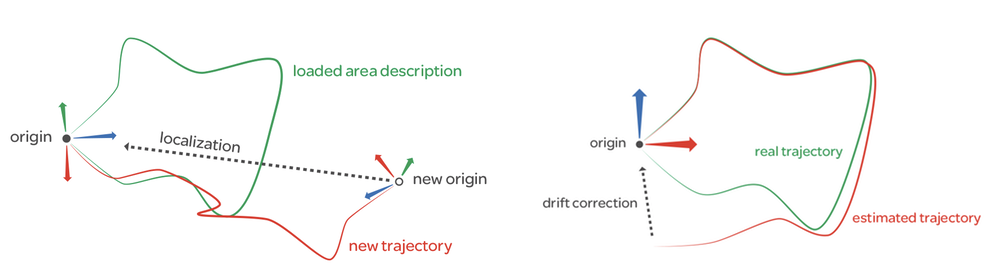
\includegraphics[width=1.0\textwidth]{content/images/theory/tango-area-learning.png} 
  \caption{Links: Lokalisierungsprozess durch Area Learning. Rechts: Korrektur von Motion Tracking anhand gelernter Merkmale. Übernommen von \citet{GoogleDevelopers:online}}
  \label{fig:area-learning}
\end{figure}

Wie bereits erwähnt entstehen bei Motion Tracking über eine längere Strecke Messfehler. 
Während diese Strecke mit einem Project Tango Gerät abgelaufen wird, ermittelt es fortlaufend die Position und den Pfad, den der Nutzer im Raum gegangen ist. 
Erkennt es während der Strecke visuelle Merkmale mittels Area Learning, wird der Pfad anhand der Positionen der Merkmale entsprechend angepasst. 
Project Tango unterscheidet hier zwischen zwei Manipulationen, \enquote{loop closures}, zur Zusammenführung des Pfads wenn ein Kreis gelaufen wurde, und \enquote{drift corrections}, um den erwähnten Drift-Effekt bei zu wenigen optischen Features im visual-inertial odometry zu korrigieren. 
Die drift correction ist in Abbildung \ref{fig:area-learning} rechts zu erkennen. \citep{GoogleDevelopersConcepts:online} 

Auch bei diesem Prozess werden die genauen Details nicht näher erläutert und es ist nicht bekannt, wie die Area Desciptions definiert sind oder was sie enthalten. \citet{GoogleDevelopersConcepts:online} weist jedoch darauf hin, dass, auch wenn die Area Desciptions Files keine direkten Bilder enthalten, es möglich sei, Rückschlüsse auf die gelernte Umgebung ziehen zu können. 

\subsection{Einordnung von Project Tango im Kontext der Augmented Reality} \label{sec:classification_project_tango}

Da sowohl die Grundlagen aus dem Bereich Augmented Reality als auch die technische Basis von Project Tango bekannt sind, kann die Project Tango Hardware bezüglich Augmented Reality näher eingeordnet werden. Bei der Hardware handelt es sich um ein hand-held Gerät, welches mit einer video see-through Display Technologie Augmented Reality Anwendungen ermöglicht. Hierfür kann wahlweise die normale RGB Kamera oder die Graustufen Fish-Eye Kamera verwendet werden. Für beide Kameras können die intrinsischen Kameraparameter ausgelesen werden, wodurch die Eigenschaften der realen Kamera durch die virtuelle Kamera übernommen werden können. Das führt zu einer parallax freien Überblendung und zu einer guten Tiefenwahrnehmung. 

Als Tracking Technologie wird hier eine hybride optische Variante angewendet. Dabei wird die Visual Odometry mit der Fish-Eye Kamera durch interne Sensoren für die Rotation, Orientierung und Bewegung kombiniert. Außerdem kann das Verfahren gegebenenfalls durch Googles Area Learning Mechanismen angereichert werden, um Messfehlern entgegenzuwirken. Die Eingabe erfolgt durch den Touchscreen des Tablets. Eine Interaktion mithilfe von optischer Gestenerkennung oder anhand der Tiefeninformationen ist zudem auch denkbar. 







% Theoretische Grundlagen
\chapter{Theoretische Vorbemerkung}

Im ersten Teil dieses Kapitels werden zunächst einmal die Grundlagen zu Augmented Reality beschrieben, wie diese Technologie einzuordnen ist, welche technischen Anforderungen ein Augmented Reality System hat und wo typische Einsatzszenarien liegen.


\section{Augmented Reality}

Augmented Reality (AR) ist eine Klasse aus dem Realitäts-Virtualitäts-Kontinuum von \cite{milgram1995augmented}, zu finden in Abbildung \ref{fig:virtual-continuum}, welche reale und virtuelle Objekte in einer realen Umgebung kombiniert. Diese virtuellen Objekte sind in der realen Umgebung idealerweise fest lokalisiert und fügen sich somit in das reale Erscheinungsbild ein. Typischerweise sind AR Anwendungen interaktiv, und stellen die virtuellen Objekte in Echtzeit und dreidimensional in der realen Welt dar. Für die Definition von AR Anwendungen gibt es zudem keine Limitierung für die Darstellungstechnologie, wie zum Beispiel das Projekt Tango Tablett oder einem Head-Mounted Display. AR beschränkt sich zudem nicht auf den angesprochenen Sinn - so sind zum Beispiel AR Anwendungen mit visueller, taktiler oder sogar olfaktorischer Umsetzung möglich.\\

Virtuel Reality (VR) oder auch Virtual Environment hingegen kapselt sich von der realen Umgebung ab und bietet Interaktionen in reinen virtuellen Umgebungen. VR konnte sich im Gegensatz zu AR deutlich schneller Entwickeln, da die technologischen Anforderungen an AR deutlich höher sind. \citep{van2010survey}\\

\begin{figure}
  \centering
	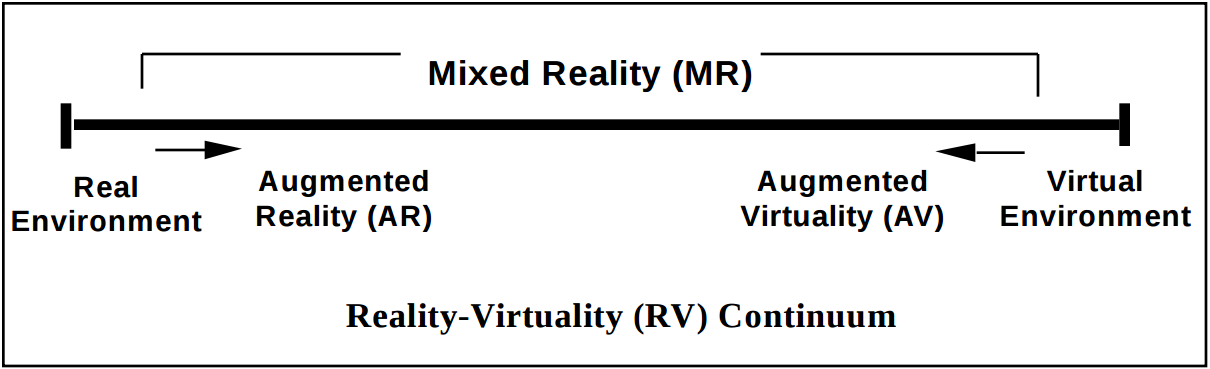
\includegraphics[width=0.85\textwidth]{content/images/theory/virtual-continuum.png} 
  \caption{Vereinfachte Darstellung des Realitäts-Virtualitäts-Kontinuum von \citet*{milgram1995augmented}}
  \label{fig:virtual-continuum}
\end{figure}

\subsection{Technische Anforderungen}

Dieser Abschnitt widmet sich den technischen Anforderungen an Augmented Reality, indem die potentiellen Display Technologien beschrieben werden, mögliche Trackingverfahren erläutern werden und zuletzt die Systeme bestimmt werden, mit denen ein Nutzer mit dem AR System interagieren kann.\\

\subsubsection{Display Technologie}

Der erste wichtige Teil der technologischen Anforderungen an AR sind visuelle Anzeigen (visual displays), welche sich nach \citet{van2010survey}
in diesem Anwendungsfall zunächst in drei Arten der Darstellung unterteilen und zudem unterschiedlich positioniert werden können. Die einfachste und günstigste Art der visuellen Darstellung in AR ist \enquote{video see-through}, wodurch die reale Umgebung durch eine Video Aufnahme ersetzt wird und die virtuellen Objekte digital in die Video Aufnahme gerendert werden. Das bietet außerdem die Möglichkeit Objekte aus der realen Umgebung zu entfernen oder zu ändern oder anhand der Luminanz Information vom Video das Rendering der virtuellen Objekte entsprechend an die Realität anzupassen.\\

Die nächste Möglichkeit zur Darstellung ist \enquote{optical see-through}, wodurch die virtuellen Objekte durch transparente Spiegel in das Sichtfeld des Betrachters gebracht werden. Anders als bei \enquote{video see-throught} bleibt die reale Auflösung für die visuelle Aufnahme des Betrachtes gleich und es können zudem keine Latenzprobleme beim Ändern des Betrachtungswinkels auftreten (parallax-effect).\\

Die dritte Möglichkeit ist die projizierte Darstellung, in der die Augmented Reality Überlagerung auf die realen Objekte projiziert werden. Diese Darstellung ermöglicht die Abdeckung vom gesamten Sichtfeld, benötigt aber eine entsprechende Kalibrierung bei Umgebungsänderungen.\\

Neben der Art der Darstellung können die Display Technologien laut \citet{azuma2001recent} anhand Ihrer Positionierung klassifiziert werden. Man unterscheidet zwischen am Kopf befestigten Displays (head-mounted), tragbare Displays (hand-held) und räumlich positionierten Displays. Zu jeder dieser Displayarten gibt es wiederum unterschiedliche technische Umsetzungen mit ihren spezifischen Vor- und Nachteilen bezüglich ihrer Anwendungsszenarien.\\

\subsubsection{Tracking Technologien}

Um eine virtuelle Projektion im realen Raum zu realisieren muss zunächst die Position und gegebenenfalls relative Positionsänderung des Displays bestimmt werden, auch \enquote{augmented reality registration} genannt. Man spricht dabei üblichweise von den \enquote{six degrees of freedom (6DOF)}, der Position im Raum (x, y, z) und der Orientierung (yaw, pitch, roll). \\

Frühe Techniken für die Registrierung benötigten üblicher Weise eine speziell vorbereitete Räumlichkeit, denn sie basierten auf mechanischen, magnetischen oder Ultraschall Sensoren um die Position zu bestimmen. Diese Sensoren sind zwar immer noch im Einsatz und bilden auch den Grundstein für AR und VR Forschung, sind aber praktisch gesehen zu komplex und aufwändig für die meisten Anwendungsfälle. \citep{van2010survey} \\

Für ein grobes Positions-Tracking, vor allem auch außerhalb von Gebäuden wird GPS genutzt. Für großräumliche Anwendung ist GPS, mit einer Varianz von 10-15 Metern und in Kombination mit einem Kompass, durchaus praktikabel. Zum Beispiel um sichtbare Flugzeuge oder Sterne visuell aufzubereiten. Innerhalb von Gebäuden basiert die grobe Positionierung laut \citet{van2010survey} oft auf verfügbaren Wifi Access Points oder RFID Markern. \citet{lamarca2005place} demonstrieren hierzu auch die Möglichkeit diese Technologie für grobe Lokalisation außerhalb von Gebäuden einzusetzen.\\

Optische Tracking Verfahren basierend auf Bildverarbeitung bieten laut \citet{van2010survey} deutlich genauere Resultate als die zuvor beschriebenen Verfahren. Es gibt hier viele verschiedene sensorische Ansätze ein optisches Tracking zu realisieren. Frühe verfahren nutzten referenzielle Marker oder Licht emittierende LEDs in einem vordefinierten Modell, um zwischen aufgenommenen Bildern eine homographische Transformation zu berechnen und um somit Rückschlüsse auf die Rotation und Positionsänderung der Kamera zu ziehen. Neue Verfahren ohne Marker nutzen Techniken zur Feature Detection und Matching um Referenzen und Bewegungen zwischen aufgenommenen Bildern zu bestimmen.\\

Viele kommerzielle und erfolgreiche Tracking Verfahren beruhen jedoch auf hybride Ansätze indem Sensoren kombiniert werden um potentielle Fehleinschätzungen eines Sensors oder einer Technik auszuschließen. So werden zum Beispiel Neigungssensor, Kompass und Gyroskop mit einem optischen Verfahren kombiniert um ein Tracking der sechs Freiheitsgrade zu optimieren. \citep{van2010survey}\\

\citet{azuma2001recent} erwähnt an dieser Stelle auch die Kalibrierung der Sensoren, die für ein präzises Registrieren nötig ist. So müssen zum Beispiel die Linseneigenschaften der Kamera für optisches Tracking bekannt sein, damit die Verfahren mit Krümmungen oder Verzerrungen umgehen können. Diese Informationen sind auch bei video see-through Displays für ein korrektes Projezieren der 3D Objekte wichtig. Zudem wird erwähnt, dass man Messfehlern oder Drifts der Position zum Beispiel mit der Zunahme von Gyroscop Informationen entgegenwirken kann, indem man auf Ereignisse wie einen Schritt des Nutzers wartet. \citep{azuma2001recent} \\

\subsubsection{Interaktions Technologien}

*

\subsection{Anwendungsbereiche}

* 


% Optimierung von AR
\chapter{Verfahren zur Realisierung von Überdeckungen in Augmented Reality durch Tiefen\-informationen} \label{sec:optimization}


Die folgenden Abschnitte widmen sich den Verfahren zur möglichen Realisierung von Überlagerungen durch Tiefen- und Bildinformationen. Nach der Recherche zu möglichen Verfahren soll erst einmal der Grundlegende Ansatz von \citet{wloka1995resolving} zur einfachen Überlagerung durch Tiefeninformationen mit Hilfe der Projektion der von Project Tango gelieferten Pointcloud realisiert werden, da dieses Ausschlussverfahren das grundlegende Vorgehensmodell zur Überlagerung darstellt. \\

Die Kanten und Modell basierenden Verfahren zur AR Überdeckung aus Kapitel \ref{sec:ar-occlusion} werden hier nicht weiter berücksichtigt, da sie offensichtliche Nachteile gegenüber anderen Ansätzen bergen. So muss bei Modell basierten Verfahren bereits ein Modell der echten Umgebung existieren und die Kanten basierte Verfahren schränkt den Einsatz auf eine weniger komplexe Szene ein. Außerdem sind beide Verfahrensarten so konzipiert, dass sie keine direkten Tiefeninformationen benötigen, die aber von Project Tango generiert werden können. Aus diesem Grund widmen sich die darauf folgend beschriebenen Umsetzung der Rekonstuktions basierten Verfahren.\\

Während dieser Arbeit wurde zunächst versucht ein eigenes Echtzeit Rekonstuktionsverfahren, basierend auf einer Ebenenerkennung zu entwickeln, welches auch auf der beschriebenen mobilen Project Tango Hardware realisierbar ist. Daraufhin wurde nach weiteren Recherchen ein neuer möglicher Rekonstruktionsmechanismus gefunden, der für den Einsatz auf mobiler Hardware konzipiert wurde. Auch dieser wird hier näher beschrieben, um ihn später zu implementieren und zu testen. Zuletzt soll näher auf die Möglichkeit eingegangen werden, die resultierenden Tiefeninformationen aus der Pointcloud oder aus dem Rendering der Rekonstruktion mit Hilfe der Bildaufnahmen der Farbkamera, zu verbessern. \\


\section{Verdeckung durch Depth Maps}

\section{Planare Rekonstruktion} \label{sec:plane-reconstruction}

Dieses Kapitel widmet sich der Idee, eine Rekonstruktion für ein  Überlagerungs\-verfahren durch eine Ebenendetektion zu realisieren. \citet{yang2010plane} erwähnen hierzu, dass Ebenen in fast allen künstlichen Umgebungen zu finden sind und aufgrund ihrer vorteilhaften geometrischen Eingenschaften in verschiedensten Computer Vision Verfahren verwendet werden. Daher gibt es viele Forschungsarbeiten, Methoden und Algorithmen, um aus verschiedensten Informationsquellen ein Ebenenmodell zu extrahieren.

Das \enquote{Simultaneous Localization and Mapping} (SLAM) Verfahren von \citet{trevor2012planar} detektiert Ebenen mit dem RANSAC Algorithmus. RANSAC bietet gegenüber anderen Algorithmen zur Ebenendetektion den Vorteil, ein Modell auch bei vielen Ausreißern performant ermitteln zu können. Agglomeratives Clustering und Region Growing wie von \citet{feng2014fast} beschrieben, eignet sich aufgrund des Ausgabeformats von Project Tango nicht direkt, da es keine organisierte Point Cloud ausgibt und die Daten durch Reflektionen und Löcher stärker mit Fehlern behaftet sind. 

Das selbst zusammengestellte Verfahren zur Ebenendetektion besteht daher aus folgenden Komponenten: Wie in dem Ansatz von \citet{yang2010plane} wird der RANSAC Algorithmus auf Würfeln ausgeführt, die eine Menge gesammelter Punkte aus der Pointcloud beinhalten. Dabei entsprechen die Würfel den untersten Knoten eines Octrees, welcher hier zur Speicherung und Aufnahme aller Punkte verwendet wird. Diese untersten Knoten des Octrees werden folgend auch Cluster genannt. Eine gefundene Ebene in einem Würfel wird wie im SLAM Verfahren von \citet{trevor2012planar} persistiert. Die Repräsentation der Ebene \(P\) wird dort wie in Gleichung \ref{eq:plane} festgehalten. Dabei handelt es sich um den Normalenvektor \(\vec{n}\) und der Distanz zum Ursprung \(d\) der Hesse Normalform einer Ebene, sowie der Punkte der konvexen Hülle \(H\). \citet{trevor2012planar} erläutern, dass die konvexe Hülle in der Repräsentation festgehalten wird, um eine sukzessive Verbesserung einer Ebene nach mehreren Messdurchläufen zu ermöglichen. So werden die Punkte der konvexen Hülle pro Messvorgang kombiniert, damit die Ebenenausbreitung auch außerhalb des Sichtfeldes beibehalten werden kann. 

\begin{equation} \label{eq:plane}
P=\left[\vec{n}, d, H\right] \qquad H=\vec{h_1}, \vec{h_2}, \ldots  \vec{h_n}
\end{equation}

Die einzelnen Schritte des Vorgehens werden in den folgenden Absätzen näher erläutert. Ein grober Ablauf des Vorgehens wird aber bereits in Listing \ref{lst:planeReconstruction} zusammengefasst und in Pseudocode beschrieben. 

\begin{lstlisting}[mathescape,caption=Planare Echtzeitrekonstruktion, label=lst:planeReconstruction, float=htbp]

Eingabe: Octree $O$, Anzahl der zu suchenden Ebene in Clustern $N$
Ausgabe: Polygonpunkte $T_{Gesamt}$

für jedes Cluster $C$=[$C_{Punkte}$, $C_{Ebenen}$] aus $O$
    führe $N$ mal aus
        bestimme Ebene [$\vec{n}$, $d$, $P$] mit RANSAC aus $C_{Punkte}$
        wenn keine Ebene mit genügend $P$ gefunden wurde
            nächstes Cluster (continue)
        wenn Ebene mit [$\vec{n}$, $d$, $H_{alt}$] in $C_{Ebenen}$ existiert	
            füge die konvexe Hülle $H_{alt}$ zu $P$ hinzu	
        bestimme die konvexe Hülle $H_{neu}$
        trianguliere $H_{neu}$ zu $T_{Ebene}$
        $T_{Gesamt}$ += $T_{Ebene}$
        $C_{Ebenen}$ += [$\vec{n}$, $d$, $H_{neu}$]
        $C_{Punkte}$ - $P$
\end{lstlisting}


\subsection{RANSAC zur Ebenendetektion} \label{sec:ransac}

Um mit dem RANSAC Algorithmus, beschrieben in Kapitel \ref{sec:ransac-theory}, Ebenen in einer Punktewolke bestimmen zu können, werden pro Iteration drei Stichproben \(\vec{A}\), \(\vec{B}\) und \(\vec{C}\) gewählt, die zur Bestimmung einer Ebene ausreichen. Das Ebenenmodell, hier in der Hesse Normalform mit dem Normalenvektor \(\vec{n}\) und dem Abstand zum Koordinatenursprung \(d\), lässt sich dabei durch die Gleichung \ref{eq:normalform} bestimmen.

\begin{equation}\label{eq:normalform}
\vec{n} =\left|\left| \vec{AB} \times \vec{AC}\right|\right|
\qquad
d = \vec{A} \cdot \vec{n}
\end{equation}

Um zu ermitteln, ob ein weiterer Punkt \(\vec{P}\) aus der Pointcloud eines Clusters die gefundene Ebene \(\left[\vec{n}, d\right]\) unterstützt, wird die kürzeste Distanz \(d_P\) zwischen Punkt und Ebene wie in Gleichung \ref{eq:plane-distance} ermittelt.  Ein entsprechender Toleranzwert für die Distanz \(d_{min}\), im gezeigten RANSAC Algorithmus \(e\) genannt, wird später bei der Umsetzung abhängig von der Ungenauigkeit des Tiefensensors gewählt. 

\begin{equation} \label{eq:plane-distance}
d_P = \vec{n} \cdot \vec{P} - d \qquad support_{d_P} = d_P < d_{min}
\end{equation}

Um das finale Modell der Ebene zu bestimmen, wie im ursprünglichen RANSAC Algorithmus in Punkt 7. aus Listing \ref{lst:planeReconstruction} beschrieben, und somit die Varianz des Abstands der Punkte zur Ebene zu minimieren, wird mithilfe der unterstützenden Punkte \(P_{s}=\left[x,y,z\right]\) eine lineare Regression durchgeführt. Diese mittelt ein Ebenenmodell \(E=\left[\vec{n}, d\right]\) aus den zuvor ermittelten Punkten mithilfe der Methode der kleinsten Quadrate. \citet{hoppe1992surface} nutzen dazu für eine ähnliche Problemstellung die Eigenwert-Dekomposition der Kovarianzmatrix der Punkte \(P_{s}\) zum Zentrum \(\vec{p_{c}}\). In Gleichung \ref{eq:centroid} wird das Zentrum aus den unterstützenden Punkten \(P_{s}\) bestimmt. Gleichung \ref{eq:covarianz} zeigt die Bestimmung der Kovarianzmatrix \(CV\) im Bezug zum Zentroid, in der \(\otimes\) für das dyadische Produkt\footnote{Wenn \(\vec{a}\) und \(\vec{b}\) die Komponenten \(a_i\) und \(b_j\) beinhalten, resultiert aus \(\vec{a} \otimes \vec{b}\) eine Matrix mit den Komponenten \(a_ib_j\) an der \(ij\) Position. \citep{hoppe1992surface}} steht.

\begin{equation} \label{eq:centroid}
\vec{p_{c}} = \frac{\sum_{n=0}^{|P|} \vec{p_{n}}}{|P|}
\end{equation}

\begin{equation} \label{eq:covarianz}
CV = \sum_{n=0}^{|P|} ( \vec{p_{n}}- \vec{p_{c}}) \otimes ( \vec{p_{n}}- \vec{p_{c}})
\end{equation}

Wendet man nun auf der Kovarianzmatrix \(CV\) die Eigenwert-Dekomposition an, erhält man die Normale \(\vec{n}\) aus dem Eigenvektor \(||\vec{v_i}||\) mit dem kleinsten Eigenwert \(\lambda_i\). Somit würde bei \(\lambda_1 \geqq \lambda_2 \geqq \lambda_3\) die Zuweisung \(\vec{n} = ||\vec{v_3}||\) folgen. Die Distanz zum Ursprung \(d\) entspricht dem Kreuzprodukt aus dem Zentroiden \(\vec{p_c}\) und der neu gewonnen Normalen \(\vec{n}\). \citep{hoppe1992surface} 

\subsection{Bestimmung der Ebenenausbreitung}

Nachdem die Ebene und die korrespondierenden Punkte zur Ebene gefunden wurden, muss noch die Ausbreitung der Fläche bestimmt werden, da die Ebene in Hesse Normalform lediglich die Position \(\vec{n} * d\) und Ausrichtung \(\vec{n}\) festhält. \citet{PlanarSurfaceMapping} nutzt hierfür die konvexe Hülle der korrespondierenden Punkte und trianguliert diese. Wie diese Triangulation genau bestimmt wird, wurde von \citet{PlanarSurfaceMapping} nicht beschrieben. 

Um diese Bestimmung performant umsetzen zu können, kann man sich die Eigenschaft der Ebene zunutze machen und die dreidimensionalen Punkte durch Parallelprojektion als zweidimensionale Punkte auf die gefundene Ebene projizieren. Denn die Triangulation ist nach dem Erhalten der zweidimensionalen konvexen Hülle, wie im Listing \ref{lst:triangulation} beschrieben, direkt bestimmbar. Nach der Triangulation können die Ecken der gefundenen Polygone jeweils zurück projiziert werden. Die Gleichungen \ref{eq:projection2d} und \ref{eq:projection3d} bilden die Projektion der Punkte wobei \(R_{\vec{n} \rightarrow \vec{z}}\) der Rotationsmatrix zwischen dem Normalenvektor \(\vec{n}\) und der Z-Achse \(\vec{z}\) entspricht.

\begin{equation} \label{eq:projection2d}
p_{2d} = (p_{3d} - (\vec{n}*d)) * R_{\vec{n} \rightarrow \vec{z}}
\end{equation}
\begin{equation} \label{eq:projection3d}
p_{3d} = (p_{2d} * R_{\vec{n} \rightarrow \vec{z}}^{-1}) + (\vec{n}*d)
\end{equation}

\begin{lstlisting}[mathescape,caption=Bestimmung der Ebenenausbreitung und Triangulation, label=lst:triangulation, float=htb]

Eingabe: Unterstützende Ebenenpunkte aus RANSAC $P$
         Transformation $R_{\vec{n} \rightarrow \vec{z}}$
Ausgabe: Polygone $T_{Ebene}$

    Projiziere alle Punkte aus $P_s$ mit $R_{\vec{n} \rightarrow \vec{z}}$ zu $P_{2d}$
    Bestimme die konvexe Hülle $H$ aus $P_{2d}$ mit Graham Scan
    starte mit leerer Menge $P_{2dmesh}$
    für $i$ von $0$ bis $|H| - 2$
        füge $H_0$ zu $P_{2dmesh}$ hinzu
        füge $H_{i+1}$ zu $P_{2dmesh}$ hinzu
        füge $H_{i+2}$ zu $P_{2dmesh}$ hinzu
    Projiziere alle Punkte aus $P_{2dmesh}$ mit $R_{\vec{n} \rightarrow \vec{z}}^{-1}$ zu $P_{3dmesh}$   
\end{lstlisting}

In Abbildung \ref{fig:polygon-process} ist der Gesamtprozess für die Bestimmung der Ebenenausbreitung veranschaulicht. Nachdem eine Ebene mit RANSAC detektiert wurde, werden die korrespondierenden Punkte auf diese zweidimensionale Ebene projiziert. Daraufhin wird die konvexe Hülle gebildet und die Triangulation der Hülle bestimmt. Diese Polygon Eckpunkte werden danach wieder zurück in den dreidimensionalen Raum projiziert.

\begin{figure}[h]
  \centering
	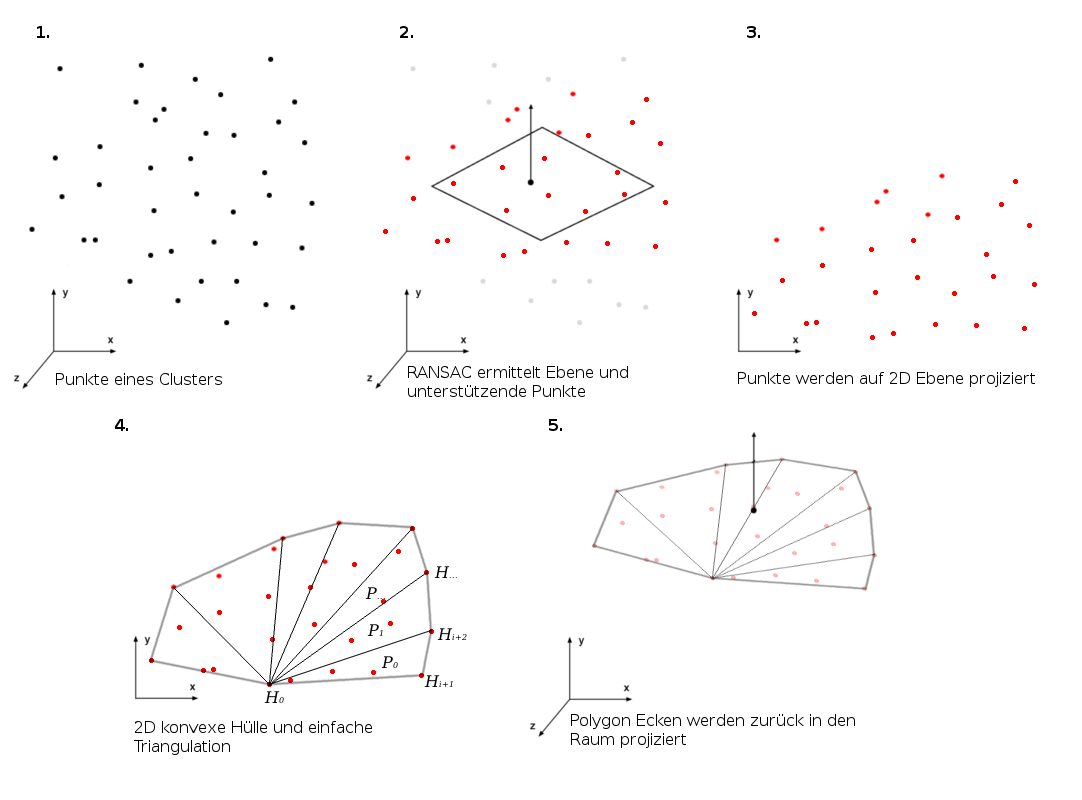
\includegraphics[width=1.1\textwidth]{content/images/methods/polygon-process.png} 
  \caption{Veranschaulichung des Gesamtprozesses zur Bestimmung der Ebenenausbreitung durch RANSAC und der konvexen Hülle.}
  \label{fig:polygon-process}
\end{figure}

\newpage

\subsection{Clustering der aufgenommenen Punkte} \label{sec:cluster}

Wie im Listing \ref{lst:planeReconstruction} zu erkennen, wird das zuvor beschriebene Vorgehen für die planare Rekonstruktion immer pro Cluster eines Cluster-Pools durchgeführt. Dadurch werden pro Durchgang des Algorithmus nur ein Bruchteil der gesammelten Punkte rekonstruiert, was wiederum eine Rekonstruktion in Echtzeit möglich macht. Außerdem verhindert das Clustering das Bilden von konvexen Hüllen über Ebenen, die in Zwischenbereichen nicht mit genügend Punkten unterstützt werden. Dieses Problem ist in Abbildung \ref{fig:clustering} links zu sehen, in welcher eine blaue Ebene rekonstruiert wird, die sich über einen Durchgang ohne vorhandene Punkte streckt.

\begin{figure}[h]
  \centering
	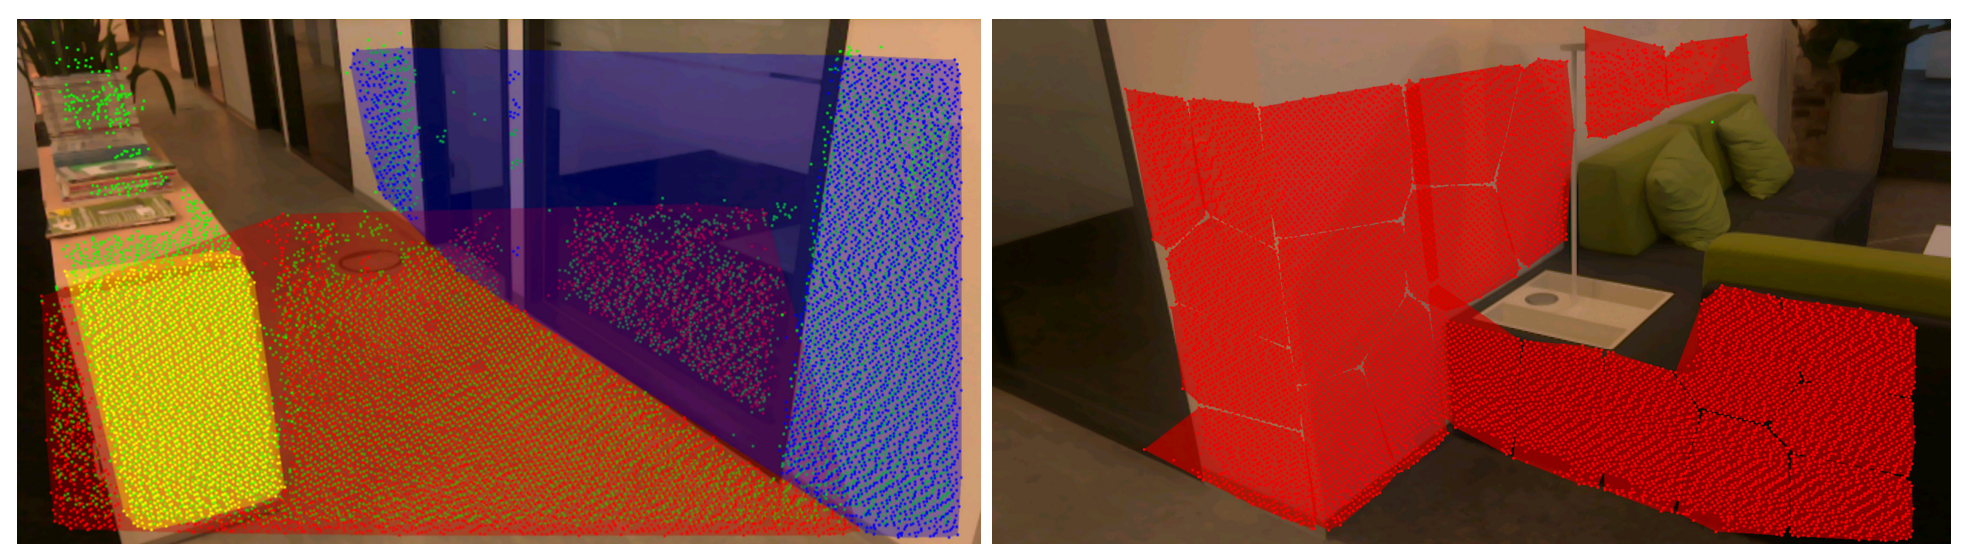
\includegraphics[width=1.0\textwidth]{content/images/methods/clustering.png} 
  \caption{Links: Ebenenrekonstruktion ohne Clustering. Rechts: Rekonstruktion mit K-Mean Clustering.}
  \label{fig:clustering}
\end{figure}

Getestet wurden hier das K-Mean Clustering, Agglomeratives Clustering und einfaches räumliches Clustern mithilfe eines Octrees. Das K-Mean Clustering hat, wie in Abbildung \ref{fig:clustering} rechts zu erkennen, gute Ergebnisse für die Aufteilung einer Ebenen geliefert, benötigt aber zuvor eine feste Anzahl von Clustern. Agglomeratives Clustering, getestet mit dem euklidischen Distanzmaß, würde zwar die Anzahl der Cluster dynamisch bestimmen, ist jedoch zu aufwändig für eine Echtzeitanwendung, wenn dieses auf die gesamten Messergebnisse durchgeführt wird. Ein Einsatz vom K-Mean oder Agglomerativen Clustering ist mangels Skalierbarkeit also nicht möglich.

Gute Ergebnisse liefert wiederum ein einfaches räumliches Clustern mit einem Octree, welcher die aufgenommenen Punkte direkt in Knoten des Baums zuweist. Das bietet zudem den Vorteil, dass diese Datenstruktur direkt als Speicherort der aufgenommenen Punkte und Ebenen dienen kann. Außerdem entspricht dies dem Vorgehen für die Anwendung von RANSAC auf Würfeln, welches von \citet{yang2010plane} beschrieben wurde. 


\section{Polygon Rekonstruktion}

\subsection{Marching Cubes}

\subsection{Possion Reconstruction}

\subsection{Greedy Projection Triangulation}



\section{Tiefenanpassungen durch Farbbilder}

Aus allen zuvor beschriebenen Verfahren werden letztendlich Tiefeninformationen, in Form von geometrischen Primitiven oder Punkten im Raum gewonnen. Diese werden passend zur aktuellen Kameraposition als Tiefenbild gerendert und füllen den Z-Buffer für eine entsprechende Aussparungen bei der Überdeckung virtueller Objekte. Auf Grund von Sensorungenauigkeiten und größeren Auflösungen der Rekonstruktionsverfahren können dabei fehlerhafte Tiefeninformationen im Z-Buffer gelangen, die zu Fehlern bei der Bestimmung der Überdeckung führen können. Dieses Problem ist am Beispiel der Pointcloud Projektion aus Kapitel \ref{sec:pc-projection} in Abbildung \ref{fig:pc-noise} zu erkennen. 

\begin{figure}[h]
  \centering
	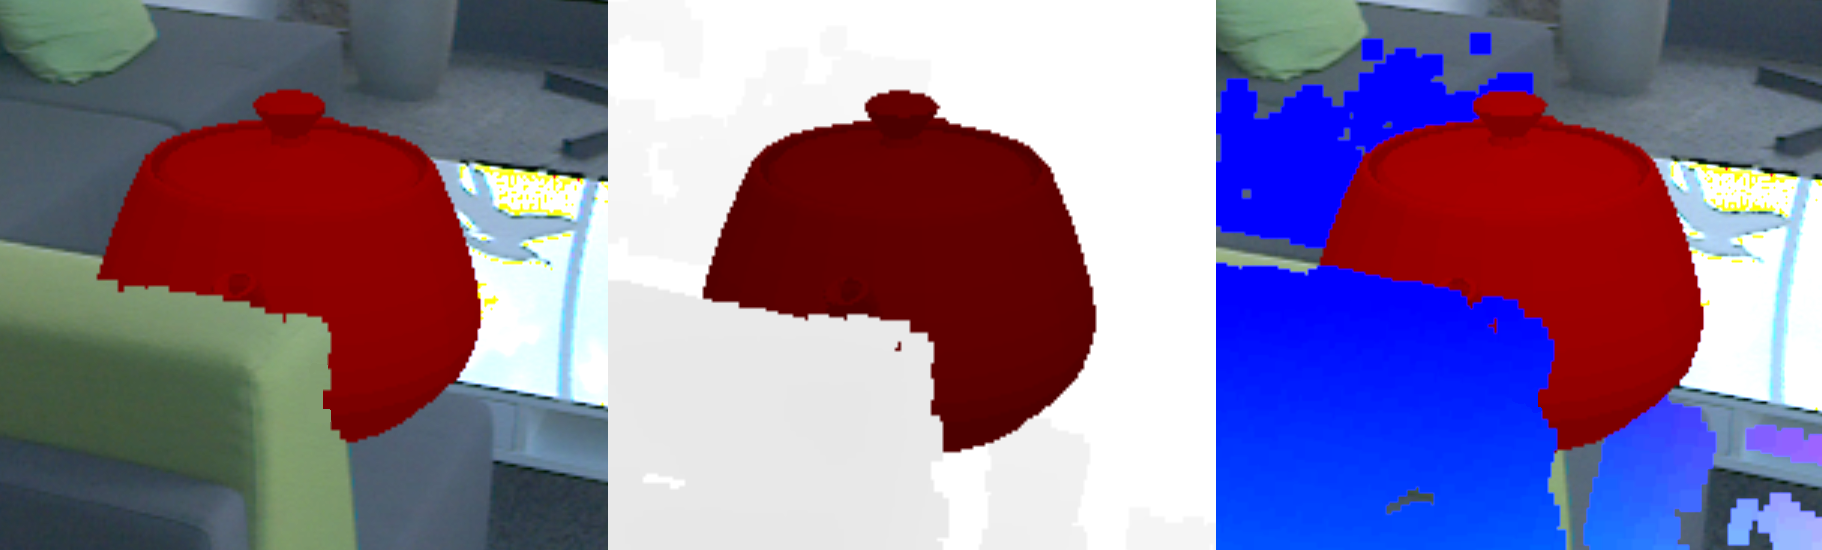
\includegraphics[width=1.0\textwidth]{content/images/methods/pc-noise.png} 
  \caption{Überdeckung mit einfacher Pointcloud Projektion. Links: Resultat der Überdeckung. Mitte: Darstellung des Tiefepuffers. Rechts: Darstellung der Pointcloud.}
  \label{fig:pc-noise}
\end{figure}

Die Reduktion von Ungenauigkeiten im Tiefenbild könnte durch einen einfachen Weichzeichner erreicht werden. Dieser würde jedoch die Kanten im Farbbild nicht berücksichtigen und somit fehlerhafte Tiefengradienten an den Kanten erzeugen und einen durchaus größeren Fehler generieren. \citet{newcombe2011kinectfusion} wenden einen sogenannten \enquote{Bilateralen Filter} in ihrem KinectFusion Rekonstruktionsverfahren an, bevor sie die Tiefeninformationen in die TSDF Repräsentation einfließen lassen. Dieser Filter von \citet{tomasi1998bilateral} ermöglicht das Weichzeichnen ohne dabei die Kanten im Bild zu übergehen, bezieht sich jedoch nur auf das selbe Bild, auf dem der Filter angewendet wird. 

\citet{liu2012guided} hingegen wenden einen sogenannten \enquote{Guided Filter} in Ihrem Verfahren zur Optimierung der der Tiefeninformationen für Kinect ähnliche Sensoren auf das Tiefenbild an. Dieser Filter von \citet{he2010guided} ist in der Lage, auf Grundlage eines anderen Leitbildes ein Weichzeichnen durchzuführen, ohne dabei die Kanten des Leitbildes zu überschreiten. Auch wenn \citet{petschnigg2004digital} eine Erweiterung, den Joint Bilateral Filter, vorstellen, der auf Basis eines anderen Leitbildes eine Weichzeichnung ohne Kantenüberschreitung ermöglicht, bietet der Guided Filter eine deutlich bessere Performance. Außerdem verhindert der Guided Filter Fehlerartefakte im Resultat, die bei dem Bilateralen Filter an den Kanten auftreten können. \citep{he2010guided} 

Ausgehend von der Eingangsgrafik \(p\), einem Leitbild \(I\) und dem Ergebnisbild \(q\) wird das grundlegende Modell dieser Art von Filter mit der Gleichung \ref{eq:gf-model} beschrieben. Diese Gleichung findet für jeden Pixel \(i\) in \(q\) eine gewichtete Summe über jeden Pixel \(j\) einer vordefinierten Ausschnittgröße. \(W_{ij}\) entspricht dabei dem Gewicht, welches für die jeweiligen Pixel \(p_j\) gilt. Bei dieser Faltung gilt üblicherweise  \(\sum_{j} W_{ij}(I)=1 \forall i \in [1\ldots |p|]\). \citep{he2010guided}

\begin{equation} \label{eq:gf-model}
q_{i} = \sum_j W_{ij}(I)p_j
\end{equation}

Der Filterkern \(W_{ij}(I)\) vom Guided Filter, zu finden in Gleichung \ref{eq:gf-W}, ist, wie auch beim bilateralen Filter, abhängig von einem Leitbild \(I\), um die Gewichte entsprechend den Kanten des Leitbildes an der Position ermitteln zu können. Die Variablen \(\mu_k\) und \(\sigma^2_k\) beschreiben jeweils den Mittelwert und die Abweichung des Leitbildes im Bildausschnitt \(w_k\). \(|w|\) entspricht der Pixelgröße des Ausschnitts. \citep{he2010guided}

\begin{equation} \label{eq:gf-W}
W_{ij}(I) = \frac{1}{|w|^2} \sum_{k:(i,j) \in w_k} (1+\frac{(I_i-\mu_k)(I_j-\mu_k)}{\sigma^2_k + \epsilon})
\end{equation}

Dieser Filterprozess wird auch als eine translationsabhänige Faltung bezeichnet, die üblicherweise aufwändig ist und dessen Berechnungsaufwand abhängig zur Filterkern Größe (\(|w|\)) ist. \citet{he2010guided} stellen jedoch noch eine andere Definition des Filters zur Verfügung, in denen alle Summen der Form \(\sum_i\in w_k f_i\) entsprechen und dadurch mit der Bildintegrationstechnik von \citet{crow1984summed} in \(O(N)\) gelöst werden können. Der Guided Filter wird in der letztendlichen Implementierung nach Gleichung \ref{eq:gf-final} implementiert, in der die Koeffizienten \(\overline{a}_i\) und \(\overline{b}_i\) dem Mittelwert über \(a_k\) aus Gleichung \ref{eq:gf-a} und \(b_k\) aus Gleichung \ref{eq:gf-b} für jedes Fenster \(w_k\) entspricht. So wird auch \(\overline{p}_k\) durch \(\frac{1}{|w|} \sum_{i \in w_k} p_i\) berechnet.

\begin{equation} \label{eq:gf-final}
q_i = \overline{a}_iI_i+\overline{b_i}
\end{equation}

\begin{equation} \label{eq:gf-a}
a_k = \frac{\frac{1}{w} \sum_{i \in w_k} I_i p_I - \mu_k \overline{p}_k}{\sigma_k^2+\epsilon}
\end{equation}

\begin{equation} \label{eq:gf-b}
b_k = \overline{p}_k - a_k\mu_k
\end{equation}

Der Faktor \(\epsilon\) reguliert im beschriebenen Filter von \citet{he2010guided} welcher Bildanteil als beizubehaltende Kante im resultierenden Bild gewertet werden soll und somit stärker oder schwächer in die Gewichtung \(W_{ij}\) Einfluss nimmt. Neben diesem Regulierungsfaktor ist auch die Wahl des Radius \(r\) für den Ausschnitt \(w_k\) als Eingabe für diesen Filter wichtig. Der Radius wirkt sich laut \citet{he2010guided} jedoch nicht wie beim bilateralen Filter auf die Laufzeit des Filters aus. 

\begin{quote}
\enquote{One more advantage of the guided filter over the bilateral filter is that it automatically has an \(O(N)\) time exact algorithm. \(O(N)\) time implies that the time complexity is independent of the window radius \(r\), so we are free to use arbitrary kernel sizes in the applications.} \citep{he2010guided}
\end{quote}

\begin{figure}[h]
  \centering
	
\includegraphics[width=1.0\textwidth]{content/images/methods/gf-result.png} 
  \caption{Guided Filter Anwendungsbeispiel. Das Tiefenbild links ergibt durch den Guided Filter mit dem Leitbild in der Mitte das Ergebnis im rechten Bild.}
  \label{fig:gf-result}
\end{figure}

Mit einer Komplexität von \(O(N)\) findet dieser Filter erfolgreich Anwendung in verschiedensten Bereichen. Er wird zum Beispiel zur Rauschunterdrückung, dem Weichzeichnen oder Verstärken von Details, zur HDR Kompression, dem Entfernen von matten Bildeigenschaften oder, wie in diesem Fall, zum zusammengeführten Anreichern von Bildinformationen verwendet \citep{he2010guided}. Angewendet auf das ermittelte Tiefenbild kann dieser Guided Filter, mit dem jeweiligen RGB Bild als Leitbild, ein Rauschen eliminieren und die Kanten der Tiefeninformationen durch ein entsprechend groß gewählten Fensterradius \(r\) und Regulierungsfaktors \(\epsilon\), an die Kanten der Kameraaufnahme angleichen \citep{liu2012guided}. Ein Beispiel für eine erfolgreiche Anwendung dieses Filters ist in Abbildung \ref{fig:gf-result} zu sehen.





% Umsetzung
\chapter{Implementierung} \label{sec:implementation}

Dieses Kapitel widmet sich der Umsetzung der in Kapitel \ref{sec:optimization} beschriebenen Verfahren. Hierfür wurden im Laufe dieser Arbeit verschiedene Prototypen entwickelt, die jeweils als Proof of Concept für die einzelnen Verfahren galten. Ziel dieser Umsetzung ist es einen einzigen Prototypen in Form einer App auf dem Project Tango Gerät zu entwickeln, die den gesamten Funktionsumfang, welcher in Kapitel \ref{sec:final_prototype} zusammengefasst wird, beinhaltet. \\

Zudem muss ein Programmfluss geschaffen werden, der es ermöglicht, in die Daten des Tiefenbuffers mit eigenen Implementierungen eingreifen zu können, um ein Filtern zu ermöglichen. Wie das technisch ermöglicht wird, und auf welcher Basis die Anwendung implementiert wird, beschreibt das Kapitel \ref{eq:technic}. Hiernach werden die Umsetzung der die jeweiligen Verfahren näher erläutert.

\section{Finaler Prototyp} \label{sec:final_prototype}

Der finale Prototyp soll, wie bereits erwähnt, alle zuvor beschriebenen Verfahren zur Realisierung von Überlagerungen in einer Augmented Reality Szene beinhalten. Also muss zunächst eine einfache AR Szene geschaffen werden, in der eine virtuelle Kamera existiert, die die intrinsischen und extrinsischen Eigenschaften der realen Project Tango Kamera zu jeder Zeit entspricht. Außerdem muss das aktuelle Farbbild der RGB Kamera in der Szene im Hintergrund dargestellt werden. Für diese Aufgaben existieren, wie bereits in Kapitel \ref{sec:theory_project_tango} erwähnt, Schnittstellen, die diese Informationen liefern. 

Um eine reale Überdeckung sinnvoll testen zu können, benötigen wir zudem ein virtuelles Objekt in der Szene. Dieses sollte im Idealfall nicht zu einfach gestaltet sein, damit die Verfahren anhand praxisnaher Gegebenheiten verglichen werden können. Zu diesem Zweck sollen Objekte in die App geladen werden können, die in dem Forschungsbereich der Computergraphik typischerweise eingesetzt werden. Typische Modelle sind zum Beispiel der \enquote{Utah Teapot}, \enquote{Stanford Bunny} oder \enquote{Blenders Suzanne}\footnote{List of common 3D test models - \url{https://goo.gl/MsOtSW} (26.02.16)}.  Eines dieser Modelle soll in die Szene geladen werden und es soll die Möglichkeit gegeben sein, dass das Objekt flexibel positioniert werden kann. Um das zu realisieren, wird der beschriebene Raypicking Mechanismus für die Auswahlgeste umgesetzt.

Um die Ergebnisse der realen Überlagerung einfach gegenüberstellen zu können, sollen die beschriebenen Tiefenbild generierenden Verfahren flexibel im Betrieb ausgetauscht werden. Dazu gehört das Rendering der Pointcloud Projektion, die TSDF Rekonstruktion durch Chisel und die Ebenenrekonstruktion. Außerdem soll das Filtern des Tiefenbildes mit Hilfe des Guided Filter optional zu jeder Zeit möglich sein. Hilfreich wäre es zudem, die Einstellungen des Guided Filters flexibel anpassen zu können. Wie diese Verfahren und der flexible Austausch umgesetzt wird, wird in den folgenden Kapiteln näher beschrieben.

\section{Technische Umsetzung und Struktur} \label{eq:technic}

Wie bereits erwähnt, basiert das Project Tango System auf Googles Android Betriebsystem. Dies ermöglicht es Anwendungen mit bestehenden und bewährten Technologien wie OpenGL, Rajawali\footnote{Android OpenGL ES 2.0/3.0 Java Engine - \url{https://goo.gl/r9Ohdj} (27.02.16)} oder der Unity Engine entwickeln zu können. Project Tango bietet hierfür drei verschiedene Schnittstellen, in C/C++, Java und Unity (Mono Framework in C\#), um auf die Sensordaten in verschiedenen Umgebungen zugreifen zu können. Im Laufe dieser Arbeit wurden alle Schnittstellen mit verschiedensten prototypischen Entwicklungen getestet.

Der finale Prototyp wurde letztendlich in C/C++ entwickelt und basiert auf dem Android NDK\footnote{Android Native Development Kit - \url{http://goo.gl/ananZT} (27.02.16)}. Außerdem greifen die anderen, höher angesiedelten Schnittstellen auf genau die selbe native Implementierung zurück, um sie in Java und Unity zur Verfügung zu stellen. Außerdem ermöglicht die native Entwicklung, neben Performancevorteilen, den vollen Zugriff auf OpenGL Mechanismen, die von Rajawali (der OpenGL Java Abstraktion) gegebenenfalls ausgeschlossen werden. 

Das Project Tango Team stellt für die native Entwicklung die eigentliche Tango Schnittstellen Bibliothek\footnote{Project Tango C API - \url{https://goo.gl/lbBfAp} (27.02.16)}, eine Support-Bibliothek\footnote{Project Tango C Suppport API - \url{https://goo.gl/VGyeKm} (27.02.16)} und eine einfache Kapselung für OpenGL Anwendungen mit dem Namen TangoGL\footnote{TangoGL Repository - \url{https://goo.gl/ymDCsJ} (27.02.16)} an. Die Support-Bibliothek bietet verschiedene Hilfsfunktionen zur Datenverarbeitung und Allokation. TangoGL wiederum erleichtert den Einstieg in die OpenGL Entwicklung und übernimmt die grundlegende Struktur und Interoperabilität zu Project Tango. Zum Beispiel gibt es Methoden, um Tango Positionsdaten in eine Translationsmatrix umrechnen zu können oder Klassen, die das Rendern der aktuellen RGB Kamera Textur übernehmen. 

Abbildung \ref{fig:structure} zeigt grob den strukturellen Aufbau der Android Applikation. Der obere Teil der Grafik bezieht sich dabei auf den in Java implementierten Teil, der die Nutzeroberfläche, ihre Interaktion und den Renderingcanvas beinhaltet. Die Activity stellt jedoch nur einen kleinen Teil der Anwendung dar, denn alle Interaktionen und Ereignisse werden über ein Java Native Interface (JNI) zum nativen Teil der Anwendung geleitet, welcher die Ansprache der Schnittstellen, die Prozesslogik und das Rendering selbst beinhaltet. 

\begin{figure}[h]
  \centering
	\includegraphics[width=1.0\textwidth]{content/images/implementation/uml.png} 
  \caption{Struktureller Aufbau des Prototypen}
  \label{fig:structure}
\end{figure}

Die Hauptklasse \enquote{ARApp} in der Grafik widmet sich in der Anwendung nur der Anreicherung und Weiterleitung von JNI Informationen und der Ansprache der Project Tango Schnittstelle. Kern der Anwendung ist die \enquote{Scene} Klasse, welche die Sensorinformationen an das entsprechend aktive Verfahren zur Tiefenbild\-generierung weiterreicht. So wird zum Beispiel die Pointcloud an das Chisel, Pointcloud oder Plane Drawable weitergereicht, damit sie ein aktualisiertes Tiefenbild rendern oder die Rekonstruktion anreichern können. Auch das Farbbild der Kamera gelangt über die Scene zum RGB Drawable, welches letztendlich als eine texturierte Fläche am Ende des Kamera Frustum dargestellt wird. Die Szene selbst ermöglicht durch den Einsatz von OpenCV\footnote{Open Source Computer Vision - \url{http://opencv.org/} (26.03.16)} den optionalen Filter Prozess durch den Guided Filter. Um das zu ermöglichen wird ein OpenGL Framebuffer eingesetzt. Die Abbildung \ref{fig:rendering-process} zeigt hierzu das Vorgehen beim Rendering der Szene mit Hilfe des zusätzlich eingesetzten Framebuffer (TB). Um den Z-Buffer Ausschluss, also die letztendliche Überlagerung zu nutzen, muss der OpenGL Depth-Test aktiviert werden.


\begin{figure}[h]
  \centering
	\includegraphics[width=1.0\textwidth]{content/images/implementation/process.png} 
  \caption{Prozessdiagramm für das Rendering der Szene}
  \label{fig:rendering-process}
\end{figure}

\section{Umsetzung der Verfahren} \label{sec:method-implementation}

\subsubsection*{Tiefe aus der Pointcloud Projektion}

Wie im Kapitel \ref{sec:pc-projection} erwähnt müssen die Punkte der Project Tango Pointcloud auf die Bildebene projiziert werden und mit einer entsprechenden Tiefenfarbe und einem Radius auf den Tiefenpuffer gezeichnet werden. Dieser Schritt wurde auch bereits in Prototoypen mit den angegebenen Gleichungen umgesetzt. 

Nach dem das Proof of Concept jedoch fertig gestellt wurde ist aufgefallen, dass OpenGL neben dem Rendering von Polygonen auch primitiven wie Punkte und Linien unterstützt. Somit konnten die Punkte im finalen Prototyp einfach vor die Kamera positioniert werden und mit Hilfe der symbolischen Konstante \enquote{GL\_POINTS} anstelle von \enquote{GL\_TRIANGLES} gerendert werden. Zudem lässt sich durch einen entsprechenden Vertexshader die Größe der Punkte anpassen. Abbildung \ref{fig:pc-demo} zeigt links die optionale gefärbte Projektion auf der Bildebene und rechts das resultierende Tiefenbild.

\begin{figure}[h]
  \centering
	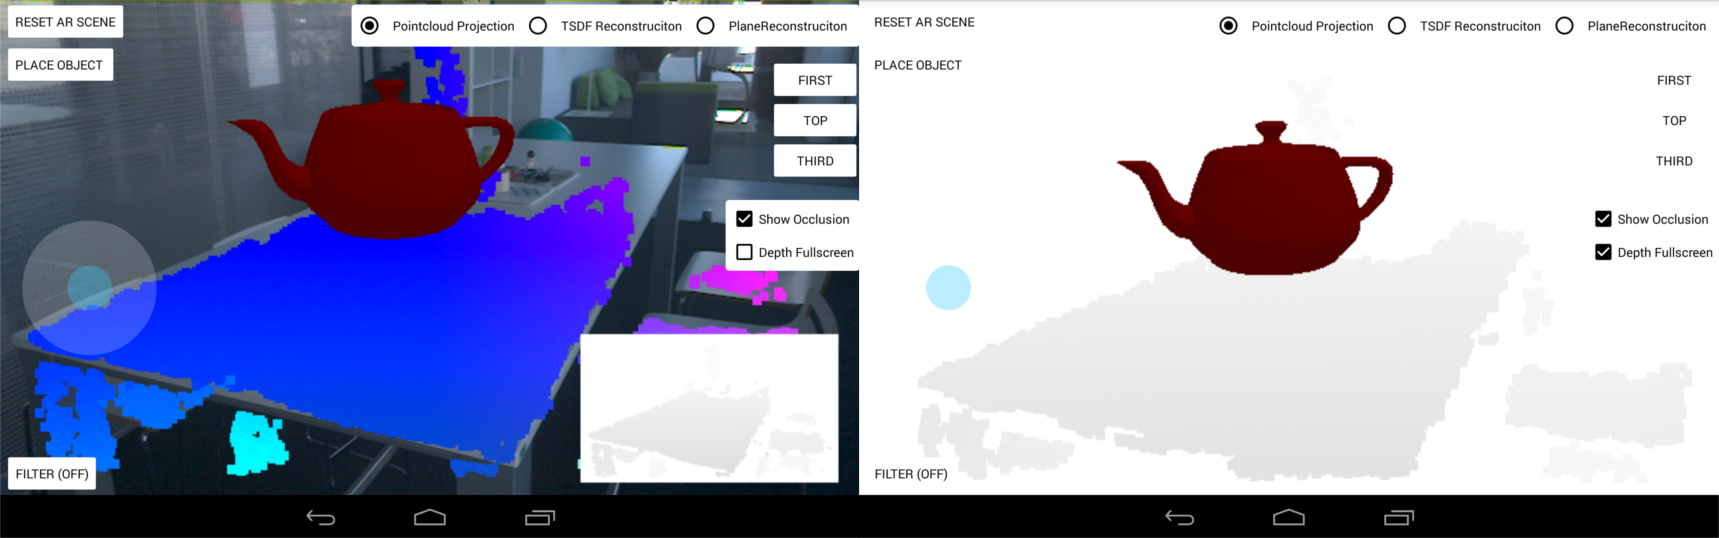
\includegraphics[width=1.0\textwidth]{content/images/implementation/pc-demo.png} 
  \caption{Pointcloud Projektion Prototyp. Links optionale Projektion auf der Bildebene. Rechts das resultierende Tiefenbild.}
  \label{fig:pc-demo}
\end{figure}



\subsubsection*{Planare Rekonstruktion}

Der erste Proof of Concept der planaren Rekonstruktion wurde zu Beginn dieser Arbeit auf Java Ebene implementiert und entwickelte sich nach und nach zu dem in \ref{sec:plane-reconstruction} beschriebenen Verfahren. Für die finale Umsetzung in dem nativen Prototypen mussten somit alle Algorithmen und Datenstrukturen neu in C/C++ umgesetzt werden. Begonnen wurde mit dem Octree, der in seinen tiefsten Zweigen die Menge aller aufgenommenen Punkte für den jeweiligen Sektor und eine Instanz der \enquote{Reconstructor} Klasse beinhaltet. Diese beinhaltet alle beschriebenen Algorithmen zur Ebenen Rekonstruktion wie RANSAC, die linearen Regression und den Graham Scan. 

\begin{figure}[h]
  \centering
	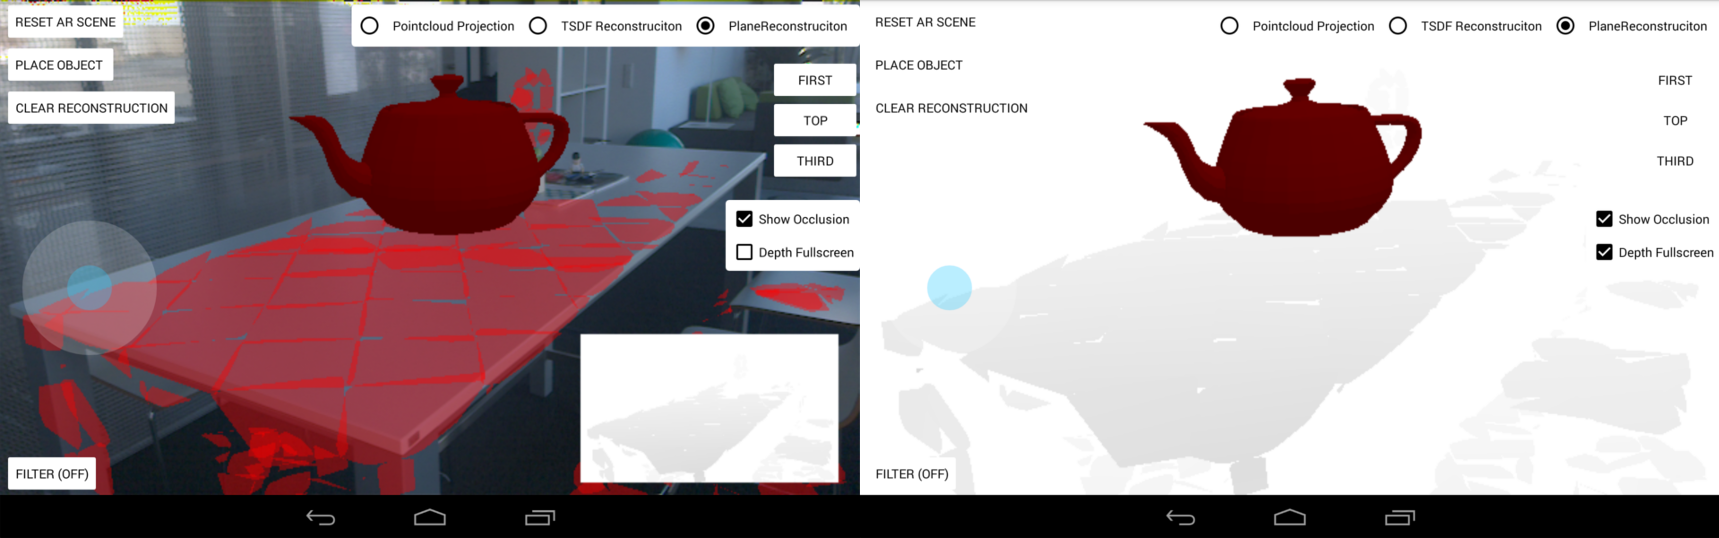
\includegraphics[width=1.0\textwidth]{content/images/implementation/plane-demo.png} 
  \caption{Planare Rekonstruktion Prototyp. Links optionale Projektion auf der Bildebene. Rechts das resultierende Tiefenbild.}
  \label{fig:plane-demo}
\end{figure}

Für die Berechnung mit Vektoren und Matrizen wurde wie auch im gesamten Projekt die OpenGL Mathematics Bibliothek (GLM)\footnote{OpenGL Mathematics - http://goo.gl/2oY83s (27.02.16)} verwendet. Sie bietet typische Primitiven mit entsprechenden Operationen für Berechnungen der linearen Algebra. Wie bereits beschrieben wird für die lineare Regression die Berechnung von Eigenvektoren mit ihren Eigenwerten benötigt. Diese Berechnung wird von GLM nicht unterstützt. Hier wurde die Eigen-Bibliothek\footnote{Eigen: template library for linear algebra - http://goo.gl/TsNOuW (27.02.16)} verwendet, die diese Operation für den Anwender anbietet. Abbildung \ref{fig:plane-demo} zeigt die Ergebnisse der Ebene Rekonstruktion links und der daraus Resultierenden Tiefeninformation rechts.


\subsubsection*{TSDF Rekonstruktion}

\citet{Klingensmith_2015_7924} erwähnen, dass ihr Verfahren Chisel zunächst als proprietäre Umsetzung im Project Tango Constructor\footnote{Project Tango Constructor - https://goo.gl/8HdTnY (27.02.16)}, Googles Demo Anwendung zur räumlichen Rekonstruktion, umgesetzt wurde. Zu Ihrer Publikation haben sie jedoch zusätzlich eine Open-Source ROS basiertes Modul zur Verfügung gestellt. Diese Bibliothek mit dem Namen OpenChisel\footnote{OpenChisel - Chisel chunked TSDF library - https://goo.gl/nla8hy (27.02.16)} wurde für den Prototypen in dieser Arbeit auf das Android NDK portiert. Dafür wurden einige Module des C++11 Standards, wie zum Beispiel \enquote{st::shared\_ptr}, die zum derzeitigen Kenntnisstand vom Android NDK nicht unterstützt oder dessen Umsetzung ein anderes Verhalten aufweist, auf die Boost\footnote{Boost C++ Libraray - http://www.boost.org/ (27.02.16)} Implementationen abgeändert. Neben der Boost Bibliothek nutzt OpenChisel auch die Eigen Bibliothek für Primitiven und Berechnungen der linearen Algebra.

Als Eingabe benötigt OpenChisel neben der Kameraposition und Kameraeigenschaften entweder einer Pointcloud oder ein Tiefenbild. In der Proof of Concept Umsetzung war erkennbar, dass OpenChisel mit der Pointcloud von Project Tango deutlich schlechtere Ergebnisse lieferte, als die Implementation des Constructors von Google. Dadurch, dass die Support Bibliothek von Google seit Februar 2016 eine performante Methode\footnote{TangoSupport\_upsampleImageNearestNeighbor - https://goo.gl/mchIie (27.02.16)} anbietet, um aus einer Punktewolke eine DepthMap mit einer Auflösung von \(320x180\) Pixel zu interpolieren, wird nun ein Tiefenbild für OpenChisel verwendet. Die resultierenden Ergebnisse kommen dadurch der Constructor Implementation deutlich näher. Abbildung \ref{fig:chisel-demo} zeigt eine exemplarische Rekonstruktion einer Pointcloud links mit dem resultierenden Tiefenbild rechts.

\begin{figure}[h]
  \centering
	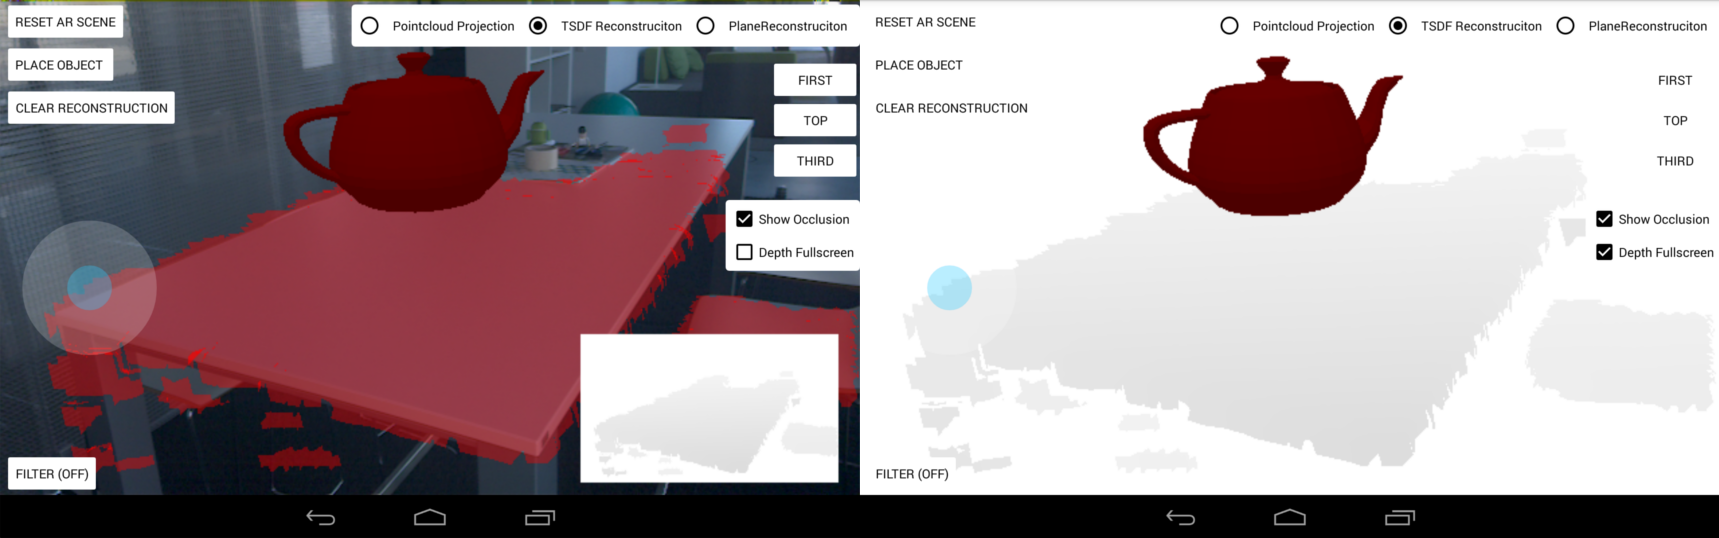
\includegraphics[width=1.0\textwidth]{content/images/implementation/chisel-demo.png} 
  \caption{OpenChisel Rekonstruktion Prototyp. Links optionale Projektion auf der Bildebene. Rechts das resultierende Tiefenbild.}
  \label{fig:chisel-demo}
\end{figure}


\subsubsection*{Guided Filter}

Für die Anwendung des Guided Filters wurde, wie bereits erwähnt, die Computer Vision Bibliothek OpenCV verwendet. Um diesen Filter mit OpenCV anwenden zu können mussten zuvor das RGB Bild und das Tiefenbild in das OpenCV Format gebracht werden. Dies war jedoch mit den Methoden \enquote{glReadPixels} und \enquote{glTexImage2D} für den aktuell selektierten Framebuffer und der OpenGL Textur problemlos möglich. Zwar sind die Speicherkonventionen von OpenGL und OpenCV, was die X und Y Achse angeht, genau vertauscht, jedoch ist das Filtern, welches daraus folgend gedreht stattfindet, für den Nutzer völlig intransparent und kann dadurch ignoriert werden.

Problematisch ist jedoch, dass das OpenGL Tiefenbild eine Farbtiefe von 16Bit nutzt und der OpenCV Guided Filter nur auf 8Bit Graustufen angewendet werden kann. Diese Transformation und die daraus resultierende Ungenauigkeit der Tiefe wurde jedoch zunächst in Kauf genommen, da erst einmal der Mechanismus als solches getestet werden soll. In der späteren Auswertung von Testszenarien muss diese Transformation berücksichtigt werden. 

Diese Implementierung ermöglicht es, den Guided Filter dynamisch auf das aktuell generierte Tiefenbild mit dem aktuell aufgenommen RGB Bild als Leitbild anzuwenden. Außerdem lassen sich die Filter Parameter, dem Radius \(r\) und den Einflussfaktor \(\epsilon\) dynamisch variieren. Abbildung \ref{fig:filter-demo} zeigt das Tiefenbild der TSDF Rekonstruktion links, auf die rechts der Guided Filter mit dem aktuellen RGB Bild angewendet wurde. 

\begin{figure}[h]
  \centering
	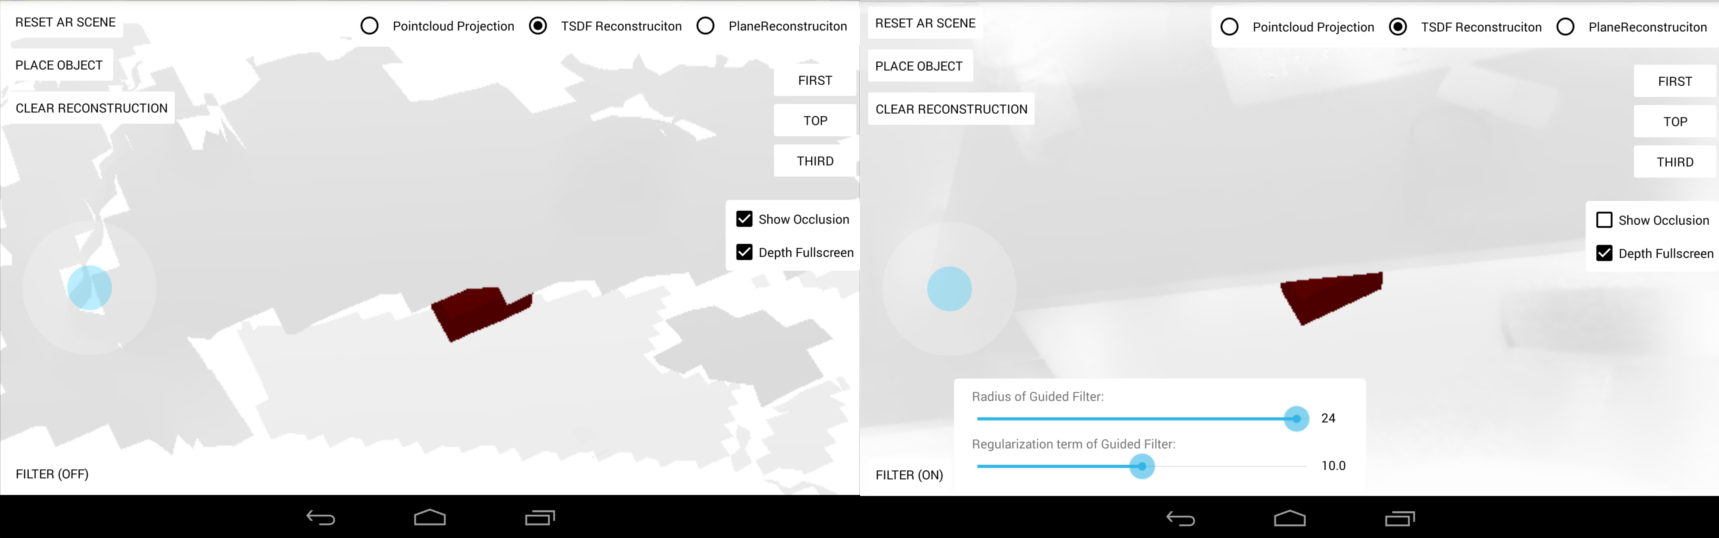
\includegraphics[width=1.0\textwidth]{content/images/implementation/filter-demo.png} 
  \caption{Anwendung des Guided Filters auf eine TSDF Rekonstruktion. Links vor und rechts nach der Anwendung.}
  \label{fig:filter-demo}
\end{figure}


\section{Technische Problemstellungen}

Auch wenn schon einige Probleme in der Umsetzung der jeweiligen Verfahren in Kapitel \ref{sec:method-implementation} näher beschrieben wurden, werden hier noch Einzelheiten aufgegriffen, die bei der Entwicklung für Projekt Tango zu beachten waren. 

Alle von Project Tango zurückgegebenen Vektoren besitzen ihre eigene Konvention bezüglich der Achsenanordnungen. Gegenüber der Konvention in OpenGL sind die Achsen \(Z\) und \(Y\) vertauscht. Außerdem zeigt die resultierende \(Z\)-Achse in die entgegengesetzte Richtung. Aufgrund dieser unterschiedlichen Konventionen müssen alle Vektoren \(\vec{v}\) von Project Tango mit der Transformationsmatrix \(T_{OGL}^{PT}\) aus Gleichung \ref{eq:transformation} konvertiert werden \citep{Proje15:online}. Nachdem Google im Laufe dieser Arbeit neue Schnittstellen\footnote{Project Tango API: Transformation Support - \url{https://goo.gl/N8dapq} (29.02.16)} zur Verfügung gestellt hat, um diese Transformationen zu abstrahieren, können die \enquote{TransformationSupport} Methoden hierfür genutzt werden.

\begin{equation} \label{eq:transformation}
T_{OGL}^{PT} =\left( \begin{matrix} 1&0&0&0\\0&0&-1&0\\0&1&0&0\\0&0&0&1 \end{matrix} \right)
\end{equation}

Wie bei vielen Echtzeitsystemen ist das Problem der Nebenläufigkeit (engl. Concurrency) auch in der Schnittstelle von Project Tango zu beachten. Die API von Project Tango publiziert die Sensordaten typischerweise asynchron. Außerdem werden die Rekonstruktionsverfahren von den entsprechenden API Publikationen angestoßen. Deshalb muss besonders beim Rendering sichergestellt werden, dass die Daten während dieses Prozesses nicht modifiziert werden. Diese Synchronisation wird durch den Einsatz von \enquote{std::mutex} aus der C/C++ Standard-Bibliothek gewährleistet. 

Bei der Anwendung des Guided Filters von OpenCV ist zu beachten, dass die  Speicherkonventionen von OpenGL und OpenCV, was die X und Y Achse angeht, genau vertauscht sind. Dadurch können zum Umwandeln der Bilder in das jeweilige Framework nicht die direkten Adressen verwendet werden, da sonst das Bild um \(90^{\circ}\) gedreht wird. Da dieser Filterprozess jedoch für den Nutzer völlig transparent durchgeführt wird und das Bild wieder in OpenCV zurück konvertiert wird, kann der Filterprozess einfach um \(90^{\circ}\) gedreht durchgeführt werden.





% Tests
\chapter{Tests} \label{sec:evaluation}

In diesem Kapitel sollen die beschriebenen und prototypisch implementierten Verfahren zur Überlagerung gegenübergestellt werden, um anhand eines direkten Vergleichs eine objektive Aussage über die Qualität der Ergebnisse treffen zu können. Hierzu wird im ersten Teil das Vorgehen zum Testen vorgestellt, welches darauf folgend mit allen Verfahren umgesetzt wird. Danach werden die daraus resultierenden Ergebnisse gegenübergestellt.

\section{Statische Testszenen}

Zum Vergleich der Verfahren wurden zwei statische Szenen gewählt, in denen das Project Tango Gerät nicht bewegt wird, um dadurch allen Kandidaten den selben sensorischen Inhalt bieten zu können. Diese Wahl auf statische Szenen wurde getroffen, um eine zuverlässige und reproduzierbare Informationsquelle für das Gerät zu schaffen. Denn die Reproduktion eines bewegten und dynamischen Szenarios ist für alle zu vergleichenden Verfahren nur sehr schwer möglich. 

Eine Idee für ein dynamisches Testszenario jedoch wäre es, alle sensorischen Informationen der Hardware während einer AR Anwendung einmal aufzunehmen und eine reproduzierbare und simulierte Umgebung dieser Daten zu schaffen. Technologien wie das Robot Operating System (ROS) würden dies ermöglichen, jedoch übersteigt der Aufwand den zeitlichen Rahmen dieser Arbeit. Auch wenn die Firma Bosch eine exemplarische Implementation\footnote{Tango Output to Rosbag Files - \url{https://goo.gl/hhnciZ} (26.03.16)} für die Aufnahme aller Daten in ROS demonstriert, sind die hier implementierten Verfahren zu sehr in den API Zyklen der Project Tango Schnittstelle involviert, um diese in kurzer Zeit auf eine Desktop Umgebung zu portieren. Um dennoch eine Aussage über die Verfahren in einer dynamischeren Anwendung treffen zu können, soll neben den statischen Tests auch manuelle dynamsiche Szenarien mit den Verfahren durchgegangen werden.

Die erste gewählte Szene, welche in Abbildung \ref{fig:static-scene} links zu sehen ist, beinhaltet einen Hocker, in Form eines einfachen  Würfels, und einen Sitzball. Der Sitzball wurde gewählt, um auch runde Formen zur Tiefenaufnahme zu testen, welche gegebenenfalls für die Verfahren schwerer zu rekonstruieren sind. Das Project Tango Gerät ist etwas höher in einem Stativ plaziert. Das virtuelle Objekt wird, wie in Abbildung \ref{fig:static-scene} rechts, zwischen die beiden realen Objekte plaziert, sodass es von beiden Seiten durch die realen Objekte überdeckt wird. 

\begin{figure}[h]
  \centering
	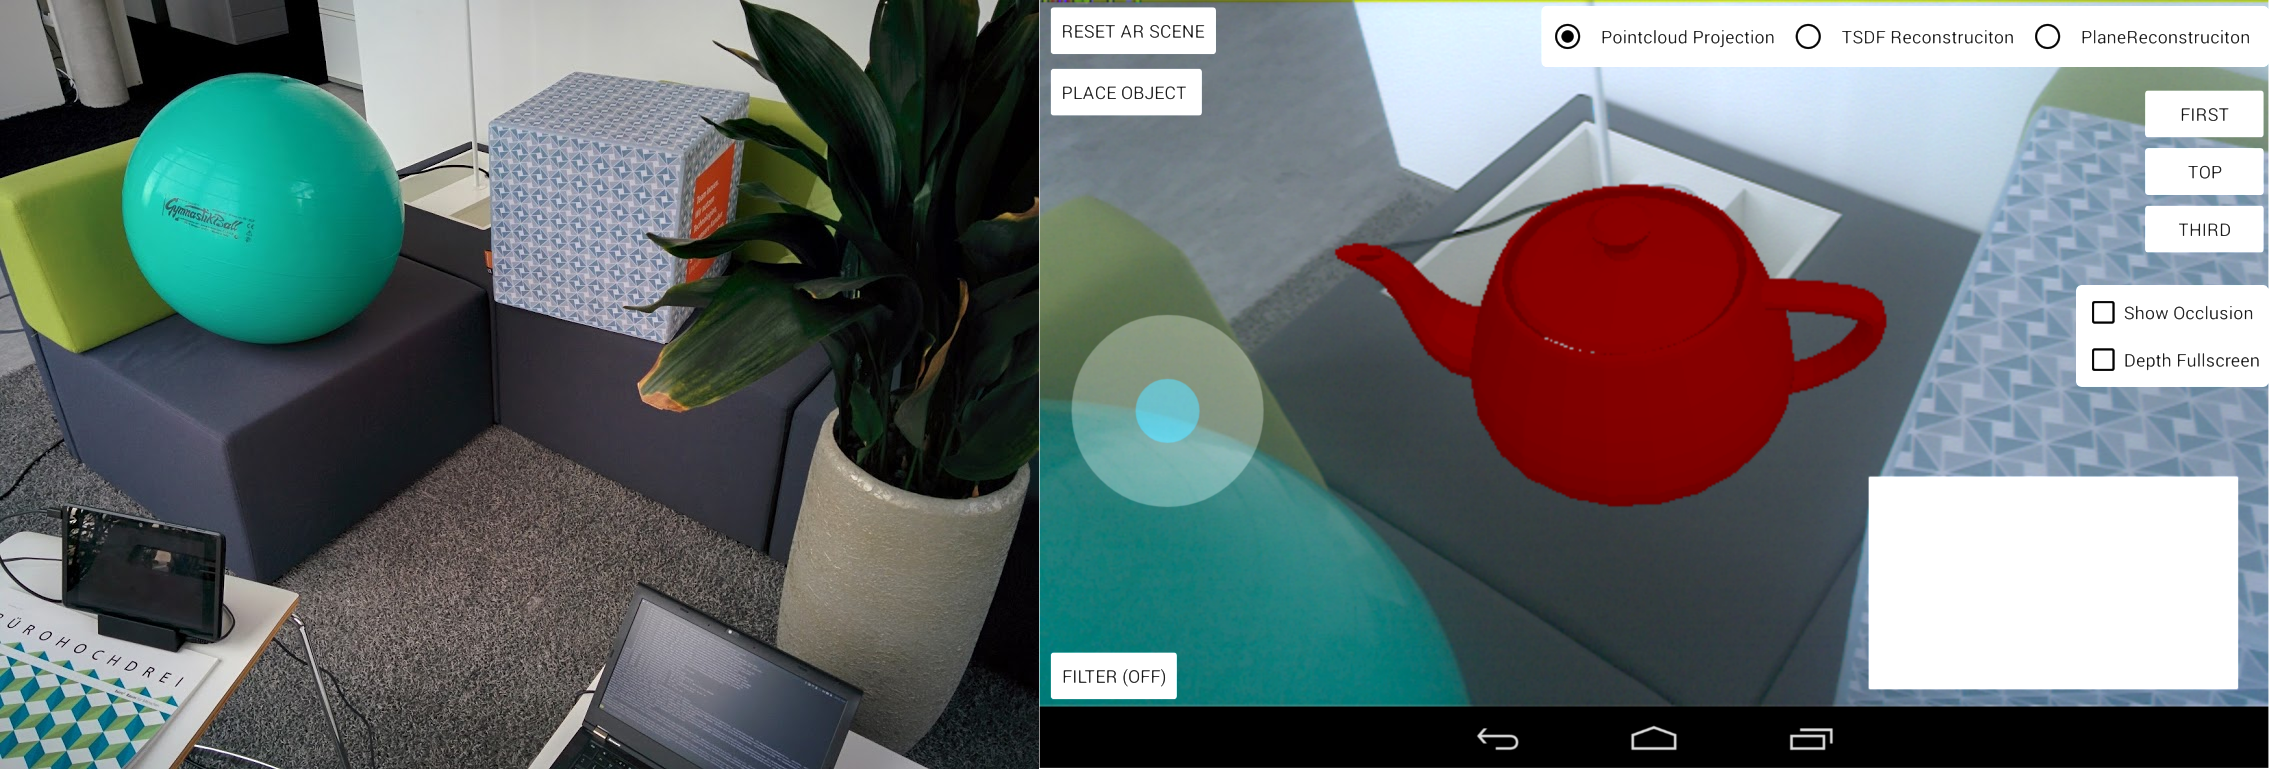
\includegraphics[width=1.0\textwidth]{content/images/evaluation/static-scene.png} 
  \caption{Links: Erste statische Szene mit einem Hocker und einem Sitzball. Rechts: Platzierung des virtuellen Objekts. }
  \label{fig:static-scene}
\end{figure}

Die zweite gewählte Szene, welche in Abbildung \ref{fig:plant-scene} links zu sehen ist, soll als Herausforderung die Überdeckung von komplexeren Strukturen testen. Sie besteht daher aus einer Pflanze, die sich, wie rechts im Bild zu sehen, vor dem virtuellen Objekt befindet. Auch hier befindet sich das Project Tango Gerät in einem Stativ, damit sich die Position während der Tests nicht ändert. 

\begin{figure}[h]
  \centering
	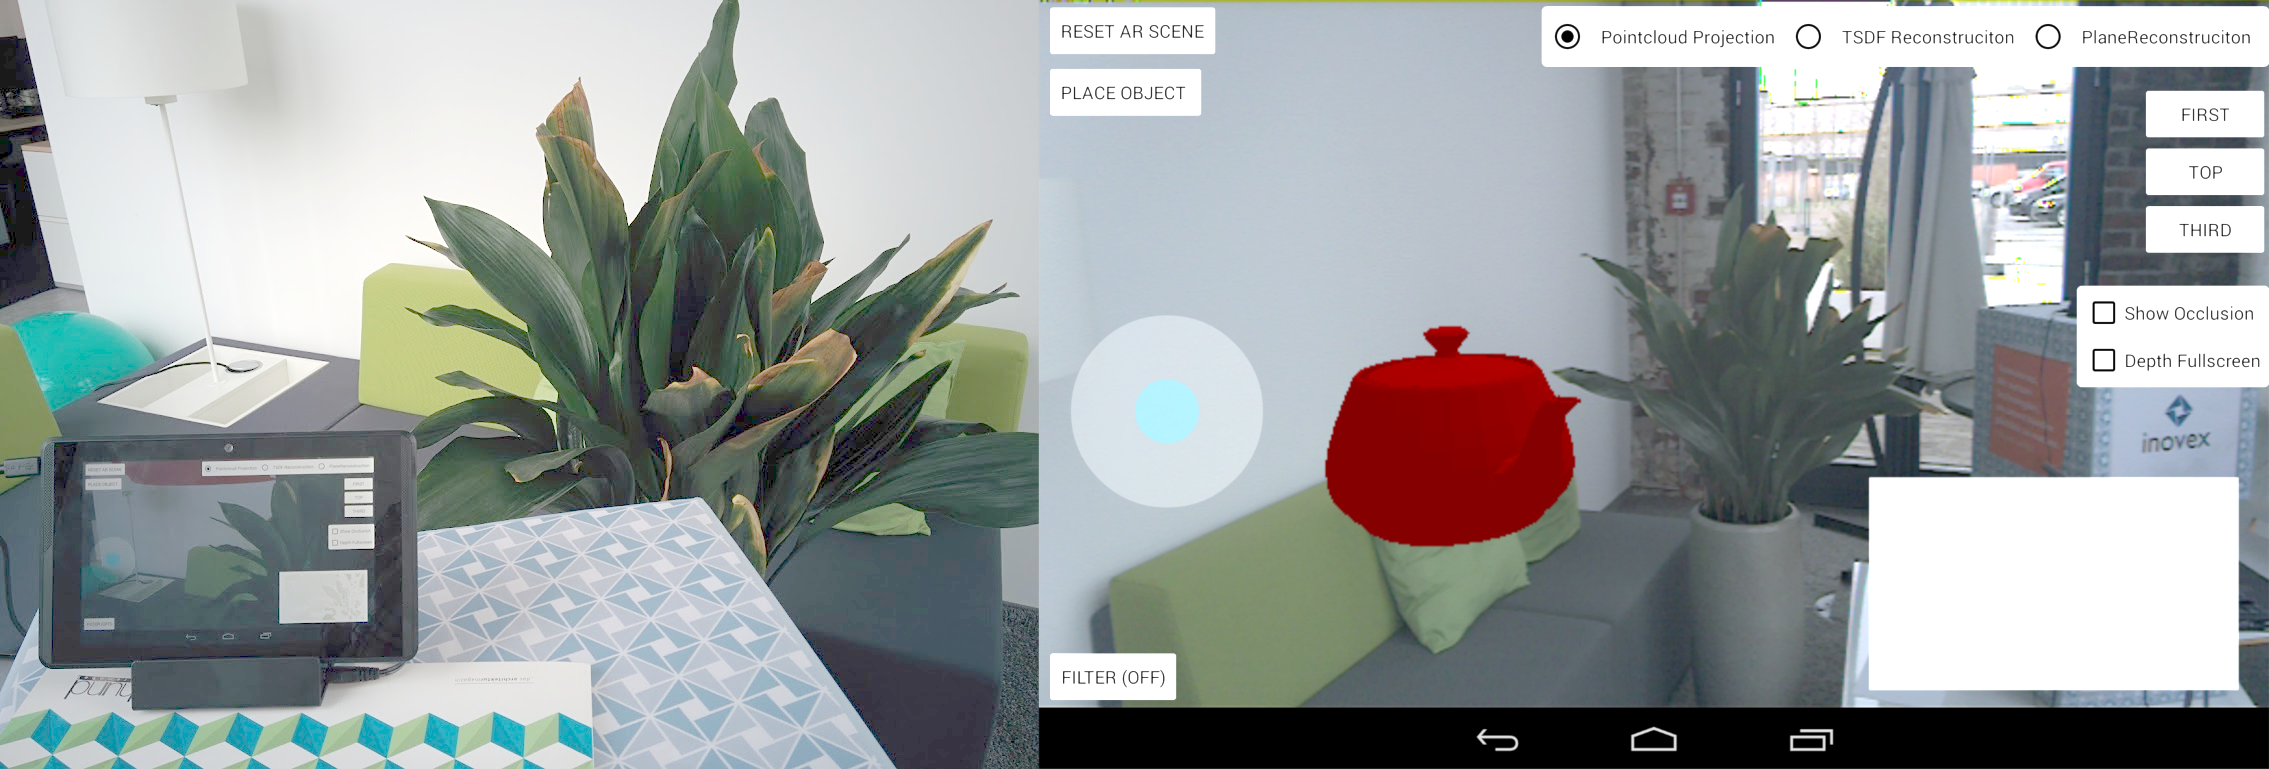
\includegraphics[width=1.0\textwidth]{content/images/evaluation/plant-scene.png} 
  \caption{Links: Zweite statische Szene mit einer Pflanze im Vordergrund. Rechts: Platzierung des virtuellen Objekts hinter der Pflanze. }
  \label{fig:plant-scene}
\end{figure}

Für beide Szenen sollen alle Kombinationen der Verfahren getestet werden. Somit ergeben sich sechs verschiedene Kombinationen pro Szene, in denen die Pointcloud Projektion, die TSDF Rekonstruktion und die Ebenenrekonstruktion jeweils mit und ohne der Anwendung des Guided Filter auf das Tiefenbild getestet werden. Für alle Kombinationen soll ein gerendertes Bild und ein Tiefenbild mit dem virtuellen Objekt festgehalten werden. Zur Auswertung werden die jeweils gerenderten Ergebnisbilder \(p\) mit einem manuell zugeschnittenem Ergebnisbild  \(q\) für jeden Pixel \(i\) verglichen. Für die Gegenüberstellung wird die Anzahl der abweichenden Pixel wie in Gleichung \ref{eq:diff} bestimmt. Ein Pixel wird nur als Veränderung gewertet, wenn die absolute Differenz der Pixel einen Faktor \(threshold\) übersteigt. Dies verhindert, dass leichte Variationen in der Farbintensität der Umgebung mit in die Wertung eingeht.

\begin{equation} \label{eq:diff}
d = \sum_i 
	\begin{cases}
		1, & \text{if } | p_i - q_i | > \text{threshold} \\
		0, & \textbf{otherwise}
	\end{cases}
\end{equation}

\section{Durchführung der Tests}

Die beiden Testszenen konnten wie beschrieben aufgebaut und mit allen Verfahren durchgetestet werden. Hierzu wurde mit der \enquote{Android Debug Bridge} (adb)\footnote{Android Debug Bridge - \url{http://goo.gl/ffH51x} (01.03.16)} eine Videoaufnahme gestartet, in der im Prototypen für jede Szene alle Verfahren durchgeschaltet wurden. Die Verfahren mussten dabei entsprechend zeitnah durchlaufen werden, um einen potentiellen Drift von Project Tangos Motion Tracking so minimal wie möglich zu halten. Denn dieser negative Effekt würden die Ergebnisse stark beeinträchtigen. 

Bei der Anwendung des Guided Filters wurde immer der Radius \(r = 24px\) und der Einflussfaktor \(\epsilon = 0.8\) gewählt. Diese Werte versprachen nach einigen manuellen Tests erfolgreiche Ergebnisse. Der Radius wurde so groß gewählt, damit die bei den Rekonstruktionen üblichen Fehler auch weitreichend in den Gewichtungskern einfließen können. Der Einflussfaktors \(\epsilon\) wurde auch größer als in den üblichen Beispielen von \citep{he2010guided} gewählten, damit nur die offensichtlich sichtbaren Kanten im Farbbild nicht vom Weichzeichnen betroffen sind. Denn ein \(\epsilon >> \sigma^2 \) für ein Bildausschnitt \(w_k\) ohne ersichtliche Kante wirkt hier wie ein zweidimensionaler Tiefpass und reduziert das Rauschen.

Abbildung \ref{fig:static_occlusion} und \ref{fig:plant_occlusion} im Anhang zeigen jeweils die aus dem Video extrahierten Bildausschnitte. Die obere Reihe zeigt die drei tiefengenerierenden Verfahren ohne den Guided Filter und die untere Reihe jeweils mit dem Filter. In der untersten Reihe sind jeweils die Projektionen der generierten Primitiven in der Szene zu sehen, um sich eine Vorstellung der Rekonstruktion machen zu können.

Nach der Ausführung dieser statischen Tests wurde jedes Verfahren zusätzlich mit einem bewegten Einsatz des Gerätes getestet. Dazu wurde das virtuelle Objekt zunächst neben einen Würfel gestellt, um danach das Gerät räumlich um den Würfel zu führen, sodass das virtuelle Objekt in der Bewegung überdeckt wurde. Da diese Tests aus zuvor beschriebenen Gründen nicht eindeutig reproduzierbar sind, werden auch keine Testdaten hiervon erhoben. Dennoch soll diese nicht rein objektive Beobachtung während dieser Tests mit in die Evaluation der Verfahren fließen.

\section{Auswertung der Ergebnisse}

Der Vergleich der Ergebnisse, welcher mit dem bereits beschriebenen Bilddifferenz Ansatz aus der Gleichung \ref{eq:diff} durchgeführt werden soll, wurde mit Hilfe der OpenCV Bibliothek durchgeführt und ist in Listing \ref{lst:compare} im Anhang zu finden. Für jede Szene wurde ein Referenzbild manuell konstruiert, welches dem idealen Ergebnis entsprechen soll. Zur Konstruktion der Vergleichsbilder wurden Ausschnitte mit leichten Anpassungen aus einigen Ergebnisbildern gewählt und zusammengeschnitten. Diese Referenzbilder sind in Abbildung \ref{fig:reference} oben zu finden. Mit dem Referenzbild wurden alle zuvor passend zugeschnitten Grafiken einer Szene verglichen. Außerdem wurde eine Maske für jede Szene für den Bereich des Ergebnisbildes bestimmt, der überhaupt für die Bestimmung der Differenz in Betracht gezogen wird. Die Masken sind jeweils in Abbildung \ref{fig:reference} unten zu finden.

\begin{figure}[h]
  \centering
	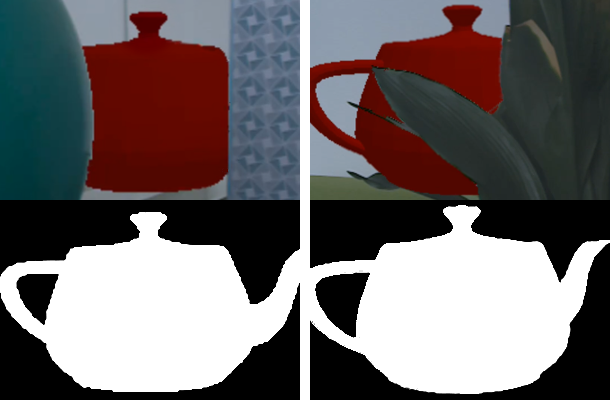
\includegraphics[width=0.7\textwidth]{content/images/evaluation/reference.png} 
  \caption{Manuell konstruierte Referenzbilder der idealen Überlagerung mit Filtermaske in Szene 1 (links) und 2 (rechts).}
  \label{fig:reference}
\end{figure}

Der gezeigte Skript zum Verglich der Ergebnisbilder mit den Referenzbildern ergibt neben den Differenzwerten, welche in Tabelle \ref{tab:results} zu finden sind, auch die absoluten Differenzbilder für jedes Verfahren. Diese Ergebnisbilder sind auch im Anhang in Abbildung \ref{fig:static_occlusion_results} zu finden. In der Abbildung werden beide Szenen mit je zwölf Bildern dargestellt, wobei jedes der drei Überlagerungsverfahren (horizontal) mit und ohne Anwendung des Guided Filter (vertikal) festgehalten sind. Sie sind also genau wie die Ergebnisse in Tabelle \ref{tab:results} angeordnet.


\begin{table}[h]
\centering
\begin{tabular}{@{}rrrr@{}}
\toprule
                      & \textbf{\begin{tabular}[c]{@{}r@{}}Pointcloud \\ Projektion\end{tabular}} & \textbf{\begin{tabular}[c]{@{}r@{}}TSDF \\ Rekonstruktion\end{tabular}} & \textbf{\begin{tabular}[c]{@{}r@{}}Ebenen \\ Rekonstruktion\end{tabular}} \\ \midrule
\textbf{Szene 1}      & 1400 & 3165 & 2193   \\
\textbf{Szene 1 + GF} & 1506 & 85 & 1545 \\
\textbf{Szene 2}      & 2478 & 4007 & 4478 \\
\textbf{Szene 2 + GF} & 67 & 1816 & 1933 \\
\bottomrule
\end{tabular}
\caption{Distanzwert zwischen dem Referenzbild und den Ergebnisbildern in der jeweiligen Szene}
\label{tab:results}
\end{table}


% Fazit
\chapter{Fazit}

* Light-Field Cameras als Kombination für AR!!

\appendix
\listoffigures
\lstlistoflistings  

\chapter{Ergebnisaufnahmen}
\begin{sidewaysfigure}[h]
  \centering
	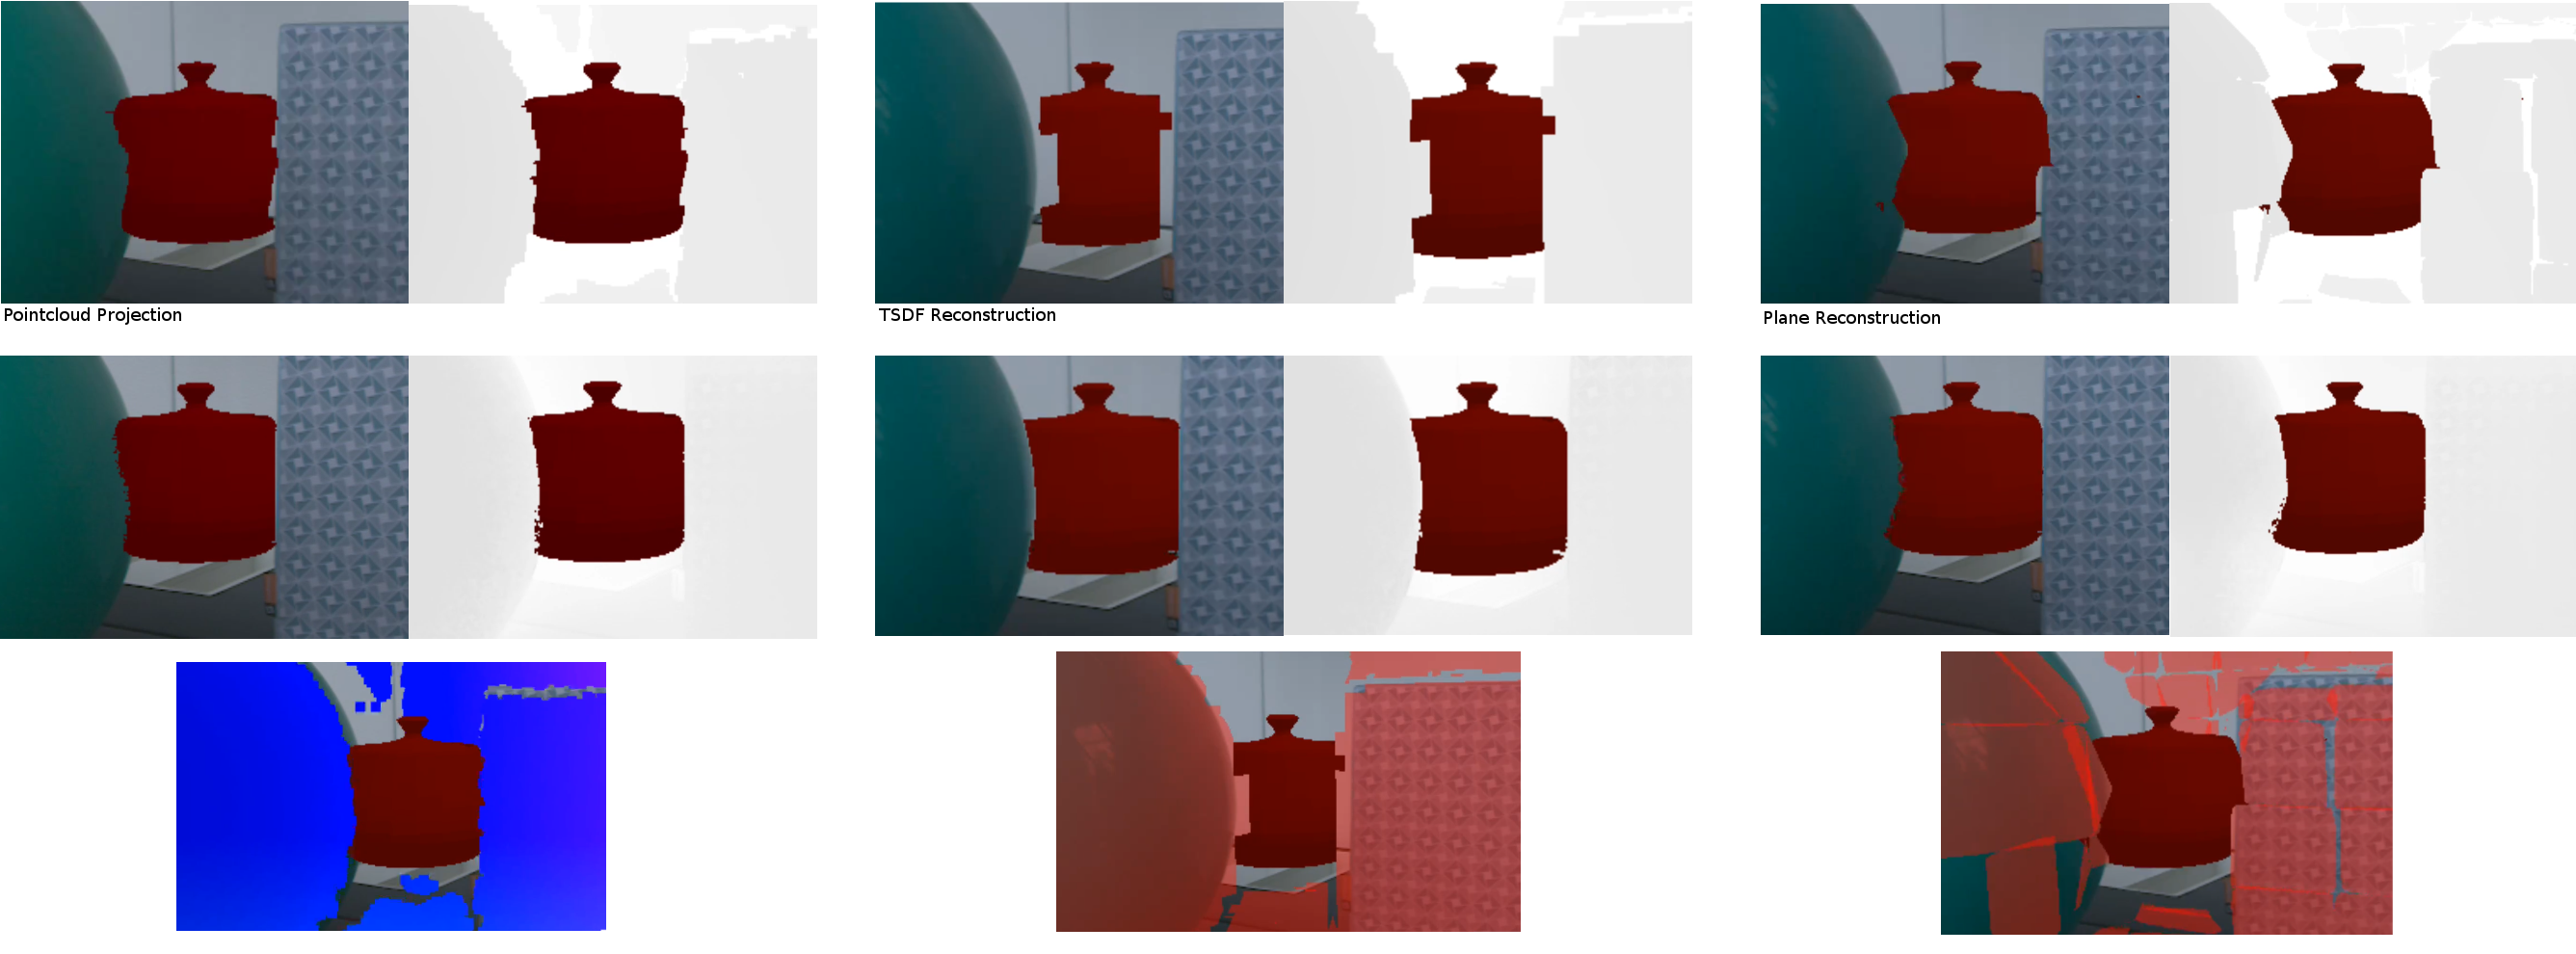
\includegraphics[width=1.0\textwidth]{content/images/evaluation/static_occlusion.png} 
  \caption{Ergebnisaufnahmen aus der ersten statischen Szene}
  \label{fig:static_occlusion}
\end{sidewaysfigure}

\begin{sidewaysfigure}[h]
  \centering
	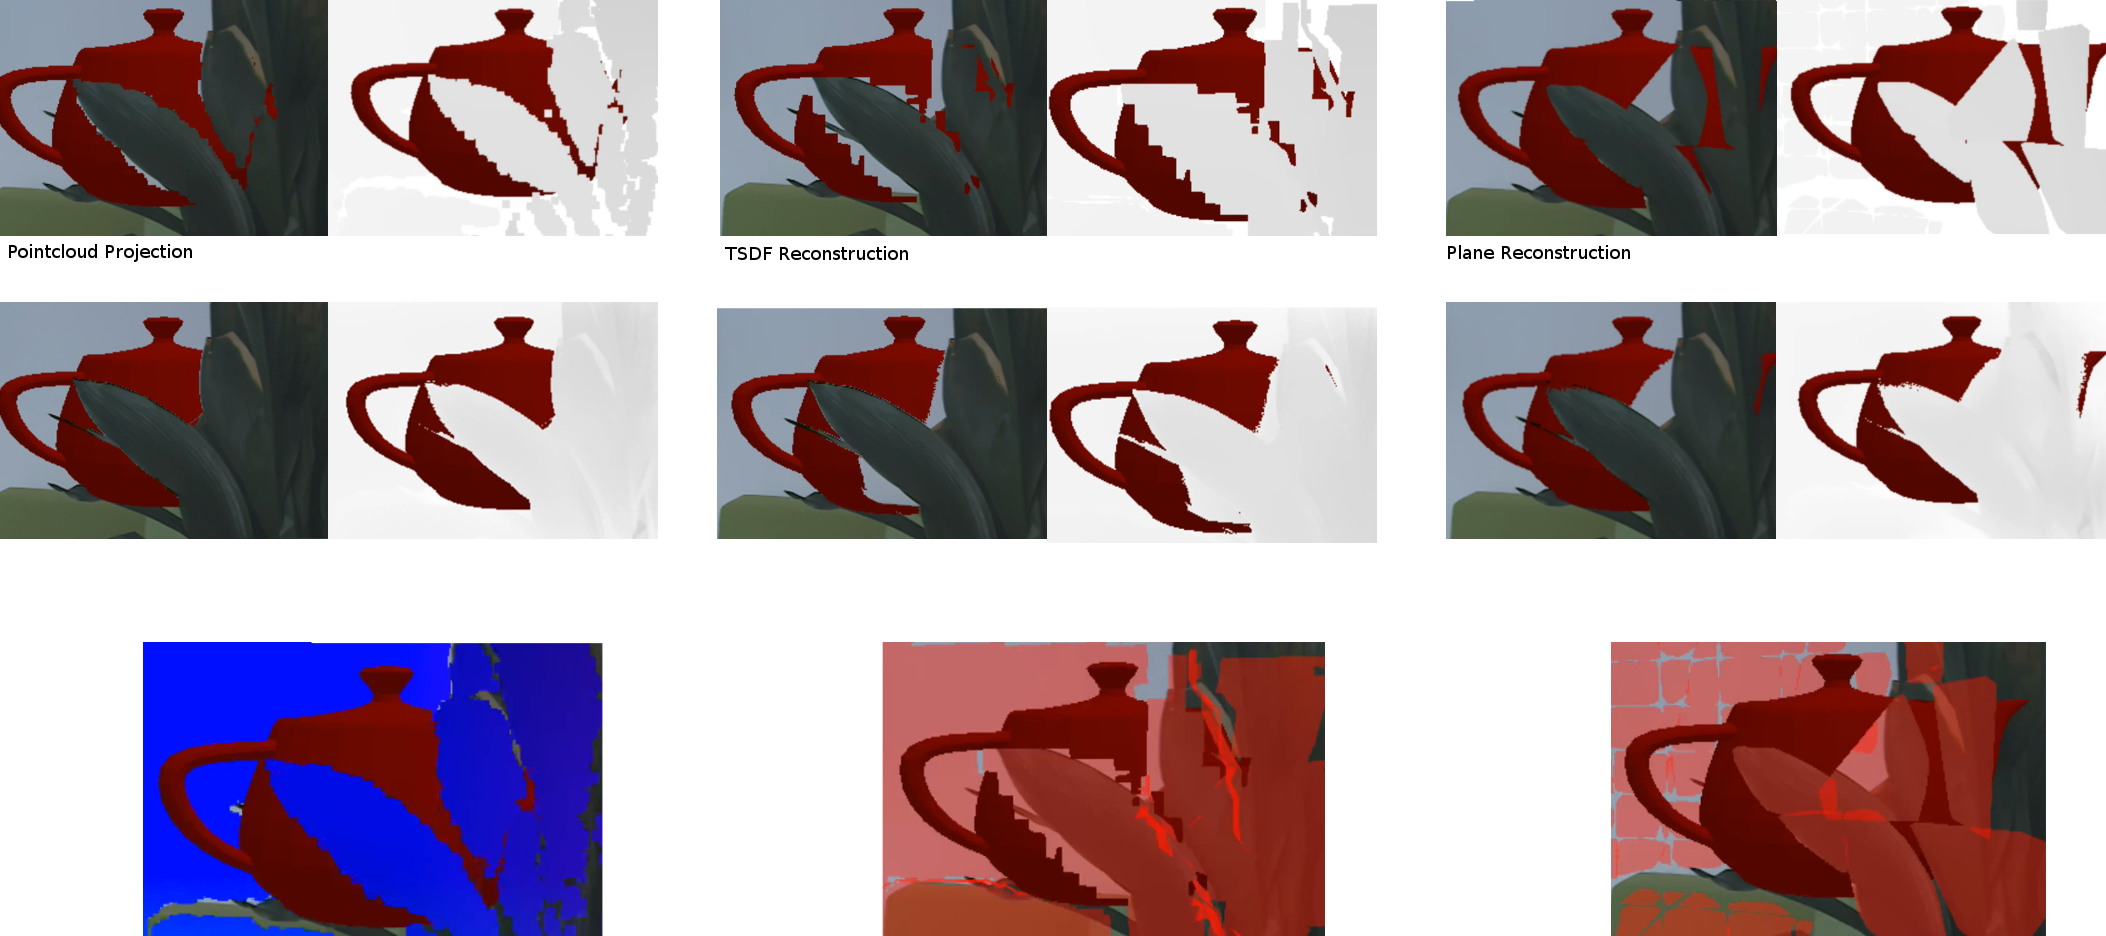
\includegraphics[width=1.0\textwidth]{content/images/evaluation/plant_occlusion.png} 
  \caption{Ergebnisaufnahmen aus der zweiten statischen Szene}
  \label{fig:plant_occlusion}
\end{sidewaysfigure}

\begin{sidewaysfigure}[h]
  \centering
	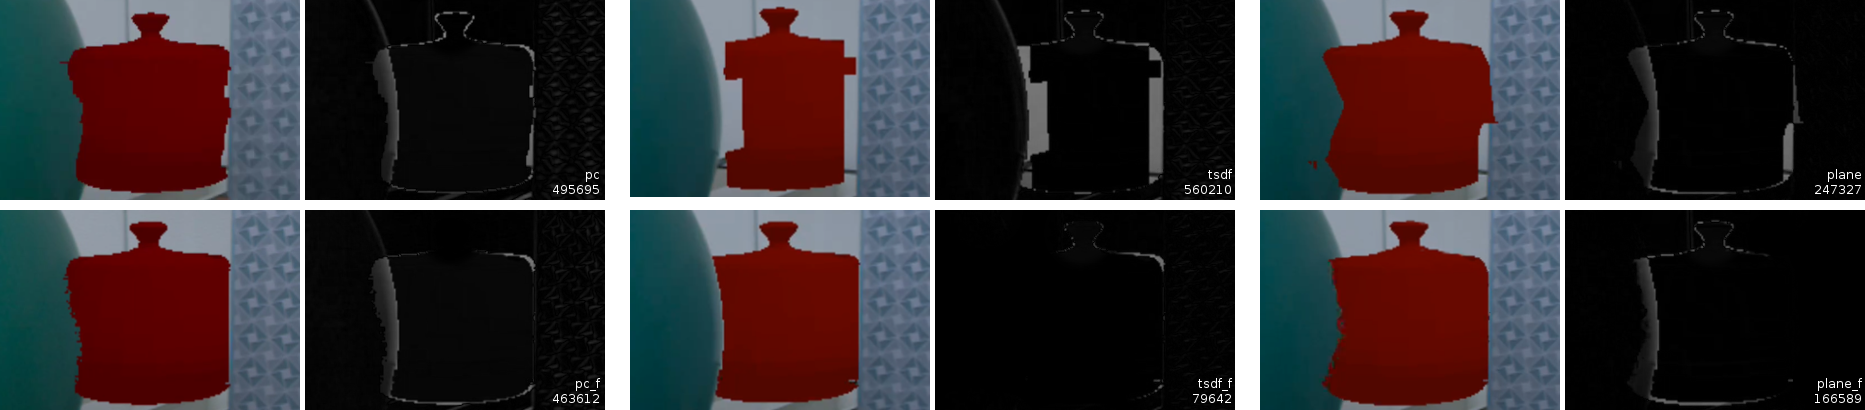
\includegraphics[width=1.0\textwidth]{content/images/evaluation/static_occlusion_results.png} 
	
\includegraphics[width=1.0\textwidth]{content/images/evaluation/spacer.png} 
	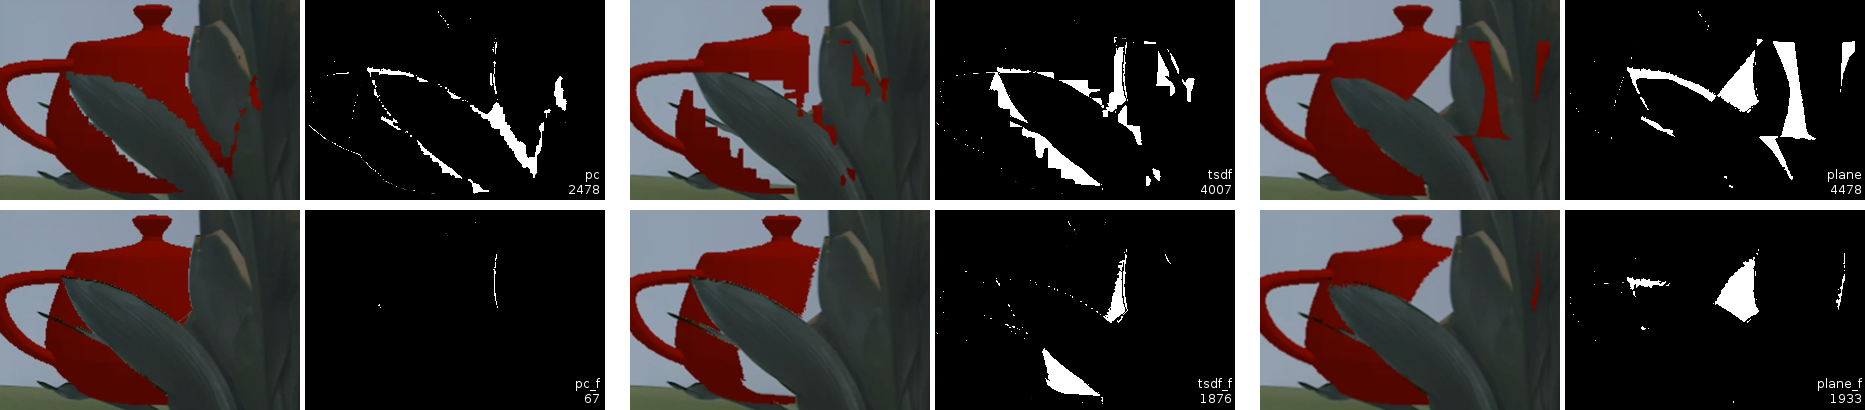
\includegraphics[width=1.0\textwidth]{content/images/evaluation/plant_occlusion_results.png} 
  \caption{Differenzbilder der Verfahren in ersten (oben) und zweiten Szene (unten)}
  \label{fig:static_occlusion_results}
\end{sidewaysfigure}


\addcontentsline{toc}{chapter}{Literaturverzeichnis}

\bibliography{main}
\bibliographystyle{natdin} 

\end{document}

